% Options for packages loaded elsewhere
\PassOptionsToPackage{unicode}{hyperref}
\PassOptionsToPackage{hyphens}{url}
%
\documentclass[
]{book}
\usepackage{amsmath,amssymb}
\usepackage{iftex}
\ifPDFTeX
  \usepackage[T1]{fontenc}
  \usepackage[utf8]{inputenc}
  \usepackage{textcomp} % provide euro and other symbols
\else % if luatex or xetex
  \usepackage{unicode-math} % this also loads fontspec
  \defaultfontfeatures{Scale=MatchLowercase}
  \defaultfontfeatures[\rmfamily]{Ligatures=TeX,Scale=1}
\fi
\usepackage{lmodern}
\ifPDFTeX\else
  % xetex/luatex font selection
\fi
% Use upquote if available, for straight quotes in verbatim environments
\IfFileExists{upquote.sty}{\usepackage{upquote}}{}
\IfFileExists{microtype.sty}{% use microtype if available
  \usepackage[]{microtype}
  \UseMicrotypeSet[protrusion]{basicmath} % disable protrusion for tt fonts
}{}
\makeatletter
\@ifundefined{KOMAClassName}{% if non-KOMA class
  \IfFileExists{parskip.sty}{%
    \usepackage{parskip}
  }{% else
    \setlength{\parindent}{0pt}
    \setlength{\parskip}{6pt plus 2pt minus 1pt}}
}{% if KOMA class
  \KOMAoptions{parskip=half}}
\makeatother
\usepackage{xcolor}
\usepackage{color}
\usepackage{fancyvrb}
\newcommand{\VerbBar}{|}
\newcommand{\VERB}{\Verb[commandchars=\\\{\}]}
\DefineVerbatimEnvironment{Highlighting}{Verbatim}{commandchars=\\\{\}}
% Add ',fontsize=\small' for more characters per line
\usepackage{framed}
\definecolor{shadecolor}{RGB}{248,248,248}
\newenvironment{Shaded}{\begin{snugshade}}{\end{snugshade}}
\newcommand{\AlertTok}[1]{\textcolor[rgb]{0.94,0.16,0.16}{#1}}
\newcommand{\AnnotationTok}[1]{\textcolor[rgb]{0.56,0.35,0.01}{\textbf{\textit{#1}}}}
\newcommand{\AttributeTok}[1]{\textcolor[rgb]{0.13,0.29,0.53}{#1}}
\newcommand{\BaseNTok}[1]{\textcolor[rgb]{0.00,0.00,0.81}{#1}}
\newcommand{\BuiltInTok}[1]{#1}
\newcommand{\CharTok}[1]{\textcolor[rgb]{0.31,0.60,0.02}{#1}}
\newcommand{\CommentTok}[1]{\textcolor[rgb]{0.56,0.35,0.01}{\textit{#1}}}
\newcommand{\CommentVarTok}[1]{\textcolor[rgb]{0.56,0.35,0.01}{\textbf{\textit{#1}}}}
\newcommand{\ConstantTok}[1]{\textcolor[rgb]{0.56,0.35,0.01}{#1}}
\newcommand{\ControlFlowTok}[1]{\textcolor[rgb]{0.13,0.29,0.53}{\textbf{#1}}}
\newcommand{\DataTypeTok}[1]{\textcolor[rgb]{0.13,0.29,0.53}{#1}}
\newcommand{\DecValTok}[1]{\textcolor[rgb]{0.00,0.00,0.81}{#1}}
\newcommand{\DocumentationTok}[1]{\textcolor[rgb]{0.56,0.35,0.01}{\textbf{\textit{#1}}}}
\newcommand{\ErrorTok}[1]{\textcolor[rgb]{0.64,0.00,0.00}{\textbf{#1}}}
\newcommand{\ExtensionTok}[1]{#1}
\newcommand{\FloatTok}[1]{\textcolor[rgb]{0.00,0.00,0.81}{#1}}
\newcommand{\FunctionTok}[1]{\textcolor[rgb]{0.13,0.29,0.53}{\textbf{#1}}}
\newcommand{\ImportTok}[1]{#1}
\newcommand{\InformationTok}[1]{\textcolor[rgb]{0.56,0.35,0.01}{\textbf{\textit{#1}}}}
\newcommand{\KeywordTok}[1]{\textcolor[rgb]{0.13,0.29,0.53}{\textbf{#1}}}
\newcommand{\NormalTok}[1]{#1}
\newcommand{\OperatorTok}[1]{\textcolor[rgb]{0.81,0.36,0.00}{\textbf{#1}}}
\newcommand{\OtherTok}[1]{\textcolor[rgb]{0.56,0.35,0.01}{#1}}
\newcommand{\PreprocessorTok}[1]{\textcolor[rgb]{0.56,0.35,0.01}{\textit{#1}}}
\newcommand{\RegionMarkerTok}[1]{#1}
\newcommand{\SpecialCharTok}[1]{\textcolor[rgb]{0.81,0.36,0.00}{\textbf{#1}}}
\newcommand{\SpecialStringTok}[1]{\textcolor[rgb]{0.31,0.60,0.02}{#1}}
\newcommand{\StringTok}[1]{\textcolor[rgb]{0.31,0.60,0.02}{#1}}
\newcommand{\VariableTok}[1]{\textcolor[rgb]{0.00,0.00,0.00}{#1}}
\newcommand{\VerbatimStringTok}[1]{\textcolor[rgb]{0.31,0.60,0.02}{#1}}
\newcommand{\WarningTok}[1]{\textcolor[rgb]{0.56,0.35,0.01}{\textbf{\textit{#1}}}}
\usepackage{longtable,booktabs,array}
\usepackage{calc} % for calculating minipage widths
% Correct order of tables after \paragraph or \subparagraph
\usepackage{etoolbox}
\makeatletter
\patchcmd\longtable{\par}{\if@noskipsec\mbox{}\fi\par}{}{}
\makeatother
% Allow footnotes in longtable head/foot
\IfFileExists{footnotehyper.sty}{\usepackage{footnotehyper}}{\usepackage{footnote}}
\makesavenoteenv{longtable}
\usepackage{graphicx}
\makeatletter
\def\maxwidth{\ifdim\Gin@nat@width>\linewidth\linewidth\else\Gin@nat@width\fi}
\def\maxheight{\ifdim\Gin@nat@height>\textheight\textheight\else\Gin@nat@height\fi}
\makeatother
% Scale images if necessary, so that they will not overflow the page
% margins by default, and it is still possible to overwrite the defaults
% using explicit options in \includegraphics[width, height, ...]{}
\setkeys{Gin}{width=\maxwidth,height=\maxheight,keepaspectratio}
% Set default figure placement to htbp
\makeatletter
\def\fps@figure{htbp}
\makeatother
\setlength{\emergencystretch}{3em} % prevent overfull lines
\providecommand{\tightlist}{%
  \setlength{\itemsep}{0pt}\setlength{\parskip}{0pt}}
\setcounter{secnumdepth}{5}
\usepackage{booktabs}
\ifLuaTeX
  \usepackage{selnolig}  % disable illegal ligatures
\fi
\usepackage[]{natbib}
\bibliographystyle{plainnat}
\usepackage{bookmark}
\IfFileExists{xurl.sty}{\usepackage{xurl}}{} % add URL line breaks if available
\urlstyle{same}
\hypersetup{
  pdftitle={A book of Practical Assignments for Psy309 at UTM Fall 2024},
  hidelinks,
  pdfcreator={LaTeX via pandoc}}

\title{A book of Practical Assignments for Psy309 at UTM Fall 2024}
\author{}
\date{\vspace{-2.5em}}

\begin{document}
\maketitle

{
\setcounter{tocdepth}{1}
\tableofcontents
}
\chapter*{About}\label{about}
\addcontentsline{toc}{chapter}{About}

This is a series of assignments intended to help third year UTM students transfer their theoretical knowledge of using the general linear model from Psy201/202 to a computational approach in \texttt{Rstudio}.

\begin{itemize}
\item
  5 ``practical'' assignments help students to refine a research question, then generate fictitious data to represent their hypothesized effect.
\item
  The final project involves synthesis of the practical assignments with additional analyses (3-way ANOVA and multiple linear regression).
\item
  As they complete the assignments, students learn to think critically about research design and construct opperationalization. They also develop basic coding skills, which are combined with their theoretical understanding of statistics in the final written assignment.
\end{itemize}

\chapter{Asking Scientific Questions and Literature Review}\label{asking-scientific-questions-and-literature-review}

\section*{Overview}\label{overview}
\addcontentsline{toc}{section}{Overview}

The purpose of this assignment is to showcase your interest in a specific topic related to psychology, and to demonstrate your ability to find \textbf{scholarly sources} that make claims related to your topic.

\textbf{\emph{Your submission should not be longer than 2 pages (including references)}}

\section*{1. Choose a Reasearch Topic in Psychology}\label{choose-a-reasearch-topic-in-psychology}
\addcontentsline{toc}{section}{1. Choose a Reasearch Topic in Psychology}

\textbf{In a single paragraph (3-5 sentences), tell us what you would like to research.}

\emph{Some questions that you could think over while selecting at topic:}

Why did you decide to study Psychology? There is some mystery about the mind, or some insight that you have had, that motivates you. Do you want to help people with a particular set of challenges? Do you want to understand growth and development? The way the brain works? How people interact? The possibilities are endless.

In this course you will learn how to develop a research proposal around a topic of your choice, one that could be the beginning of a grant proposal or a way to wow potential supervisors for grad school, or to impress potential employers who want to know if you can lead project. The more you make this something relevant to your own goals, the more useful this course will be.

It must be a topic in \emph{psychology}: i.e., the study of the mind, and it should be something that can be studied \emph{scientifically}, i.e., observed in such a way that other people could replicate your process and generate similar data. This topic will be the basis for your research project over the course of the semester, so please give it some thought!

\section*{2. See What's Out There}\label{see-whats-out-there}
\addcontentsline{toc}{section}{2. See What's Out There}

Go to \href{https://guides.library.utoronto.ca/psycinfoovid}{the library PsycINFO page}, \href{https://scholar.google.ca/}{Google Scholar}, or similar academic search engine.

Conduct a basic search for a topic that you are interested in. If you would like more information about this process, we have multiple videos on conducting a literature search available online.

\textbf{Please write a few paragraphs describing:}

\begin{itemize}
\item
  The search engine(s) that you used
\item
  What were the \emph{specific} search terms you used (so if we entered those terms, we should get the same output as you)
\item
  How did you expand / change your search terms to focus on the types of studies you were most interested in?
\item
  Provide a reference list of 3-5 peer-reviewed, academic research papers on your research topic; the references should be listed in \href{https://guides.library.utoronto.ca/c.php?g=250462&p=1670709}{APA format}.
\item
  At least one of your papers must be an empirical paper!
\end{itemize}

\textbf{Provide a brief (3-5 sentence) summary of one empirical, peer-reviewed research paper from your list} (preferably one that represents an approach to your research topic that you find interesting.)

\begin{itemize}
\tightlist
\item
  Tell us what the paper was about and why you chose it - how did you know it was an empirical paper? What about it was interesting to you?

  \begin{itemize}
  \tightlist
  \item
    You don't have to tell us everything about the paper- again just a 3-5 sentence summary in your own words, which means you must leave many details out! You will get into the details of this paper in the next two practical assignments. Note: you can change this `focus paper' later if you find something better, but it is better to start with a specific paper in mind.
  \item
    You will end up having to create an empirical research proposal by the end of the term, so this paper can be an important example for you to rely and build upon as the term goes on. The important thing is to pick a paper and dive in - this is a `safe space' to just immerse yourself in a research approach, regardless of whether you actually perform research like this in the future!
  \end{itemize}
\end{itemize}

\section*{3. Reflect}\label{reflect}
\addcontentsline{toc}{section}{3. Reflect}

\textbf{Write a closing paragraph (3-5 sentences) describing what it was like to try to find research on your topic.}

\begin{itemize}
\tightlist
\item
  Was it hard to pick a topic? Did your topic change based on what you found (or couldn't find) during your literature review? What advice would you give to other students doing this assignment in the future?
\end{itemize}

\chapter{Exploring Types of Measurement in Research}\label{exploring-types-of-measurement-in-research}

Unlike other ways of knowing (epistemologies), the scientific method requires that we specify a way of measuring things in the world. It is important that the specified set of methods is described in such a way that other people could \emph{replicate} the experiment, assuming that they have access to the necessary resources and training.

\section*{1. Identify dependent variable(s)}\label{identify-dependent-variables}
\addcontentsline{toc}{section}{1. Identify dependent variable(s)}

Think back to your submission from practical \#1 (where you selected a general research topic and found some articles, with at least one of the articles performing empirical measurement).

Remind us about the research topic that you have chosen to focus on. This time, \textbf{use a \emph{single sentence} that cites the empirical article in APA style}. Please also provide the full citation for the paper as well, in APA format (make sure that the components of the citation are written using APA standard, but \textbf{do not worry} about formatting the citation with a hanging indent).

For example:

\begin{quote}
On the topic of factors people's enjoyment of meditation, researchers have observed that while most people expect to enjoy breath-focused meditation more than visualization or mantra practices, but approximately half of all participants change their minds after trying all three practices (Anderson \& Farb, 2018).
\end{quote}

\begin{quote}
Anderson, T., \& Farb, N. A. (2018). Personalizing practice using preferences for meditation anchor modality. \emph{Frontiers in psychology}, \emph{9}, 1-10.
\end{quote}

\textbf{Describe the primary dependent variable in the research paper}. Remember that a \emph{dependent variable} is something that is observed (or measured), and is outside of the researcher's direct control (i.e., the dependent variable is not manipulated). If your paper has multiple dependent variables, you can mention that, but please tell us which variable you consider to be the most important.

\section*{2. Identify claim(s) made by the paper}\label{identify-claims-made-by-the-paper}
\addcontentsline{toc}{section}{2. Identify claim(s) made by the paper}

One of the main reasons that we measure things is to make a claim about a broader population or about future events. Remember that the three main types of claims we make are: \emph{frequency}, \emph{association}, or \emph{causal} claims. Make sure that you connect the DV to the IV(s) here to explain the parameters of the research finding.

\textbf{Describe which of the three claims is / are being made} in the paper that you outlined above and explain how you know (i.e., your reasoning). Could the DV be used to make the other two types of claims? What sort of study would be needed for each?

\section*{3. Critically Evaluate the Measuement Approach}\label{critically-evaluate-the-measuement-approach}
\addcontentsline{toc}{section}{3. Critically Evaluate the Measuement Approach}

In class and in the textbook, we have begun to explore the idea that not all measures are equally \emph{valid} and \emph{reliable} for making inferences. We discussed four forms of validity in class: construct, statistical, internal, and external.

Consider the validity of the empirical paper that you have selected. Please \textbf{define each of the four validities in your own words} using 1-2 sentences each. Then \textbf{write 3-4 sentences discussing the validity of the paper}. You may not feel super confident on the statistical validity, but you can discuss the others. For example, does the dependent variable accurately represent the construct that you are interested in exploring? Does the way they studied the construct make sense? Do the data come from a sample that has a good chance of generalizing to other people and other situations?

\section*{4. Develop a Research Idea}\label{develop-a-research-idea}
\addcontentsline{toc}{section}{4. Develop a Research Idea}

Now that you have reviewed the kinds of studies that are published in your field of interest and taken a look a the types of variables they use, expand on the existing work. \textbf{Write 2-3 paragraphs describing a novel study idea} that would produce data to support at least two of the ``types of claims'' that we have discussed in class (e.g., Frequency AND Association). Make sure that you clearly describe the independent and dependent variables in the study.

What ideas do you have, either about re-using a measure you've read about, or improving / creating a new measure to investigate your topic? What sort of inference are you hoping to make? To describe something that we know little about? To look at the relationship between two or more constructs? Or to show that changing something about the situation causes changes in your dependent variable?

Please specify the \textbf{rationale} for the study (why would this research be important?), the \textbf{primary research question} (what is the primary thing these data will tell you?) and the \textbf{hypothesis} / \textbf{predicted results} (what sort of results are you predicting and WHY?).

\section*{5. Reflect}\label{reflect-1}
\addcontentsline{toc}{section}{5. Reflect}

\textbf{Write a closing paragraph (3-5 sentences) describing how you are thinking about measuring the construct of interest in your research topic}. Remember that we will be creating and analyzing fictitious data over the next few weeks to further explore the research process. Would the study that you are conceptualizing be feasible in the real world? Why or why not? What processes would you need to follow in order to actually conduct this study (e.g., REB approval..)

\emph{Submissions should be 2-3 pages in length. References don't need to be written on a separate page. No marks for APA format, so please feel free to make use of various levels of headings to enhance readability.}

\chapter{Manipulations and Covariates}\label{manipulations-and-covariates}

\section*{1. Connecting covariates to your topic of interest}\label{connecting-covariates-to-your-topic-of-interest}
\addcontentsline{toc}{section}{1. Connecting covariates to your topic of interest}

By this point, you've had a chance to develop your ideas around how to measure a construct within your research topic of interest. The simplest thing to do with such information is just to report its properties, like the average grade in a class, or frequencies, like how many people sign up for different classes. These are known as descriptive statistics.

But if we want to go further and understand why the world is the way that it is, we may try to see how things we can measure are linked together. If we are going to observe more than one variable of interest and see how closely linked these variables are, we are beginning to engage association claims, which often involves a \emph{correlational} approach. When one variable is correlated with another variable of interest, we call it a \emph{covariate}.

For your topic of interest, \textbf{describe a second construct / covariate that you suspect is linked (either positively or negatively) to your main variable of interest}. What is your reasoning for selecting this variable? Is there an obvious reason that it is relevant, or, even better- is it mentioned as being related in the research literature? \textbf{In a short paragraph (3-5 sentences), describe:}

\begin{itemize}
\tightlist
\item
  Discuss your idea for why the two variables might be related.
\item
  Be clear if the proposed relationship is positive or negative, and speculate about the strength.
\end{itemize}

\begin{figure}
\centering
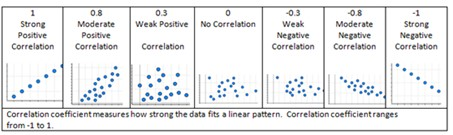
\includegraphics{Figs/strength.jpg}
\caption{\label{fig:unnamed-chunk-1}Figure 1. A reminder about the data patterns that correspond to various correlation coefficients}
\end{figure}

\begin{itemize}
\tightlist
\item
  Provide an in-text citation to (at least) one peer-reviewed article that shows that the constructs might be related.

  \begin{itemize}
  \tightlist
  \item
    If there is no direct evidence or reporting of this relationship, then cite an article that shows that show some sort of peripheral evidence that could support the relationship that you are proposing.
  \end{itemize}
\item
  Below the paragraph, provide an APA style reference to the paper that you cited.
\end{itemize}

\section*{2. Experiments: Manipulating Independent Variable(s)}\label{experiments-manipulating-independent-variables}
\addcontentsline{toc}{section}{2. Experiments: Manipulating Independent Variable(s)}

If we want to go further from just showing an association to establishing that one construct directly influences or \emph{causes} changes in another, we need to do experiments. In an experiments, we \emph{manipulate} one variable to see if those unpredictable/independent manipulations create predictable effects on the dependent variable.

Think of a way in which you could manipulate an independent variable to create changes in your dependent variable of interest. In a short paragraph (3-5 sentences):

\begin{itemize}
\tightlist
\item
  Discuss your idea for how you could manipulate one thing (the independent variable) to change the dependent variable.
\item
  Be clear on the direction of manipulation, e.g., if one increases how much an assignment is worth, a student's nervous level will also increase
\item
  Provide an in-text citation to (at least) one peer-reviewed article that shows that the constructs might be related. If you can't find evidence of the exact same manipulation, show an association and describe how you could change it into a manipulation, or show how the manipulation has been used in another context but could be applied here.
\item
  If there is no direct evidence or reporting of this relationship, then cite an article that shows that these constructs could be related.
\item
  Below the paragraph, provide an APA style reference to the paper that you cited.
\end{itemize}

\section*{3. Connect the theory to computation in R!}\label{connect-the-theory-to-computation-in-r}
\addcontentsline{toc}{section}{3. Connect the theory to computation in R!}

\textbf{Generate} an example mock data set that includes the variables that you described in part 2 (above) with 100 participants per group. \textbf{Print out a nice looking table that shows} the \textbf{n}, \textbf{mean}, \textbf{min}, \textbf{max}, and \textbf{standard error of the mean} for the key dependent variable that you are interested in measuring. Make sure that your table is organized to show these descriptive statistics for each of the experimental conditions that you proposed in part (2) above.

\begin{itemize}
\item
  Creating a reproducible data set will require using functions in \texttt{Rstudio}. For this reason \textbf{\emph{this assignment must be generated using \texttt{Rstudio}}}.
\item
  Make sure to watch Jennet's videos (on Quercus) about how to generate data and tables through \texttt{Rstudio}.
\item
  Make sure that you have \texttt{echo\ =\ TRUE,\ warning\ =\ FALSE,\ message\ =\ FALSE} set for your code blocks so that the output shows your code, but not the messages or warnings that R sends (and watch the tutorial video to get info on what this means).

  \begin{itemize}
  \tightlist
  \item
    Don't print the whole data-set that you've created in-line, or your output document will be really long.
  \end{itemize}
\end{itemize}

\section*{4. Reflect}\label{reflect-2}
\addcontentsline{toc}{section}{4. Reflect}

Write a closing paragraph (3-5 sentences) summarizing what it is like learning to work with R and what it is like to see all the variables visualized. What questions and/or difficulties have arisen? Do you think it is helpful to be able to simulate your data ahead of time? What do you think about the group size of n = 100 (e.g., should it be increased or decreased?).

Additionally, feel free to reflect on the process of using Rstudio to generate data - Is there anything that would have improved your experience doing this lab?

\section*{Code For Practical \#3}\label{code-for-practical-3}
\addcontentsline{toc}{section}{Code For Practical \#3}

\subsection*{Object-oriented programming}\label{object-oriented-programming}
\addcontentsline{toc}{subsection}{Object-oriented programming}

Examples of how Rstudio can be used to assign single values, lists of values, or 2-D arrays of Data.

\begin{Shaded}
\begin{Highlighting}[]
\CommentTok{\# Notes }

\CommentTok{\# text will cause problems }

\CommentTok{\# First example }

\DecValTok{67} \SpecialCharTok{*} \DecValTok{88}
\end{Highlighting}
\end{Shaded}

\begin{verbatim}
## [1] 5896
\end{verbatim}

\begin{Shaded}
\begin{Highlighting}[]
\CommentTok{\# Object{-}oriented programming }

\NormalTok{a }\OtherTok{\textless{}{-}} \DecValTok{67} \SpecialCharTok{*} \DecValTok{88} \CommentTok{\# Assign the result of the function onto the object "a"}

\CommentTok{\# Example 2 }

\NormalTok{b }\OtherTok{\textless{}{-}} \FunctionTok{c}\NormalTok{(}\DecValTok{1}\NormalTok{,}\DecValTok{2}\NormalTok{,}\DecValTok{3}\NormalTok{,}\DecValTok{4}\NormalTok{,}\DecValTok{5}\NormalTok{) }\CommentTok{\# Assign a list onto the object "b"}

\CommentTok{\# Example 3 {-} DATA FAME }

\NormalTok{c }\OtherTok{\textless{}{-}} \FunctionTok{data.frame}\NormalTok{( }\CommentTok{\# Assign a 2{-}D data frame onto the object "c"}
  \AttributeTok{ID =} \FunctionTok{c}\NormalTok{(}\DecValTok{1}\NormalTok{,}\DecValTok{2}\NormalTok{,}\DecValTok{3}\NormalTok{,}\DecValTok{4}\NormalTok{,}\DecValTok{5}\NormalTok{), }
  \AttributeTok{Score =} \FunctionTok{c}\NormalTok{(}\DecValTok{100}\NormalTok{,}\DecValTok{110}\NormalTok{,}\DecValTok{90}\NormalTok{,}\DecValTok{95}\NormalTok{,}\DecValTok{107}\NormalTok{)}
\NormalTok{)}
\end{Highlighting}
\end{Shaded}

\subsection*{Random number generation}\label{random-number-generation}
\addcontentsline{toc}{subsection}{Random number generation}

\begin{Shaded}
\begin{Highlighting}[]
\FunctionTok{set.seed}\NormalTok{(}\DecValTok{123}\NormalTok{) }\CommentTok{\# Beginning of the random process}

\NormalTok{d }\OtherTok{\textless{}{-}} \FunctionTok{data.frame}\NormalTok{(}
  \AttributeTok{ID =} \FunctionTok{c}\NormalTok{(}\DecValTok{1}\SpecialCharTok{:}\DecValTok{100}\NormalTok{), }\CommentTok{\# 100 IDs}
  \AttributeTok{Score =} \FunctionTok{runif}\NormalTok{(}\AttributeTok{n=}\DecValTok{100}\NormalTok{,}\AttributeTok{min=}\DecValTok{1}\NormalTok{,}\AttributeTok{max=}\DecValTok{10}\NormalTok{) }\CommentTok{\# 100 random scores}
\NormalTok{)}

\FunctionTok{head}\NormalTok{(d) }\CommentTok{\# show me the first 6 rows}
\end{Highlighting}
\end{Shaded}

\begin{verbatim}
##   ID    Score
## 1  1 3.588198
## 2  2 8.094746
## 3  3 4.680792
## 4  4 8.947157
## 5  5 9.464206
## 6  6 1.410008
\end{verbatim}

\begin{Shaded}
\begin{Highlighting}[]
\FunctionTok{tail}\NormalTok{(d) }\CommentTok{\# show me the last 6 rows}
\end{Highlighting}
\end{Shaded}

\begin{verbatim}
##      ID    Score
## 95   95 3.883359
## 96   96 2.689220
## 97   97 8.040649
## 98   98 1.842355
## 99   99 5.201011
## 100 100 5.603549
\end{verbatim}

\begin{Shaded}
\begin{Highlighting}[]
\FunctionTok{hist}\NormalTok{(d}\SpecialCharTok{$}\NormalTok{Score, }\AttributeTok{xlab =} \StringTok{"Random value (x)"}\NormalTok{, }\AttributeTok{col =} \StringTok{"grey"}\NormalTok{, }\AttributeTok{main =} \StringTok{""}\NormalTok{, }\AttributeTok{cex.lab =} \FloatTok{1.5}\NormalTok{, }\AttributeTok{cex.axis =} \FloatTok{1.5}\NormalTok{) }\CommentTok{\# print out a quick histogram of the data}
\end{Highlighting}
\end{Shaded}

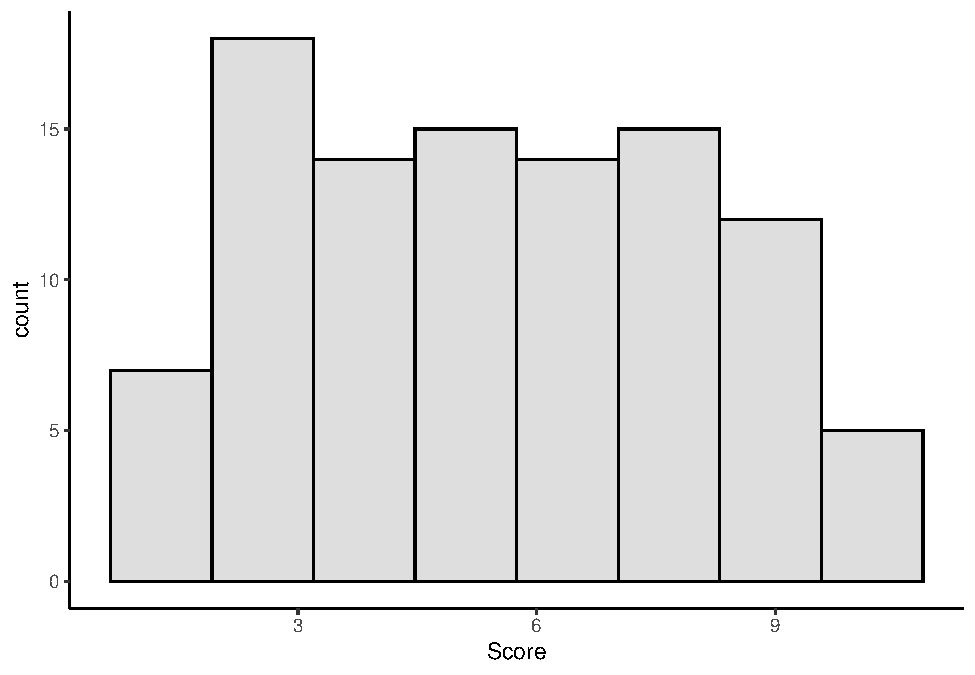
\includegraphics{_main_files/figure-latex/unnamed-chunk-4-1.pdf}

\subsection*{Sample from the normal distribution}\label{sample-from-the-normal-distribution}
\addcontentsline{toc}{subsection}{Sample from the normal distribution}

\begin{Shaded}
\begin{Highlighting}[]
\NormalTok{e }\OtherTok{\textless{}{-}} \FunctionTok{data.frame}\NormalTok{(}
  \AttributeTok{ID =} \FunctionTok{c}\NormalTok{(}\DecValTok{1}\SpecialCharTok{:}\DecValTok{100}\NormalTok{),}
  \AttributeTok{Score =} \FunctionTok{rnorm}\NormalTok{(}\AttributeTok{n =} \DecValTok{100}\NormalTok{, }\AttributeTok{mean =} \DecValTok{100}\NormalTok{, }\AttributeTok{sd =} \DecValTok{15}\NormalTok{) }\CommentTok{\# sample from normal distribution}
\NormalTok{)}

\FunctionTok{hist}\NormalTok{(e}\SpecialCharTok{$}\NormalTok{Score, }\AttributeTok{xlab =} \StringTok{"Random value (x)"}\NormalTok{, }\AttributeTok{col =} \StringTok{"grey"}\NormalTok{, }\AttributeTok{main =} \StringTok{""}\NormalTok{, }\AttributeTok{cex.lab =} \FloatTok{1.5}\NormalTok{, }\AttributeTok{cex.axis =} \FloatTok{1.5}\NormalTok{)}
\end{Highlighting}
\end{Shaded}

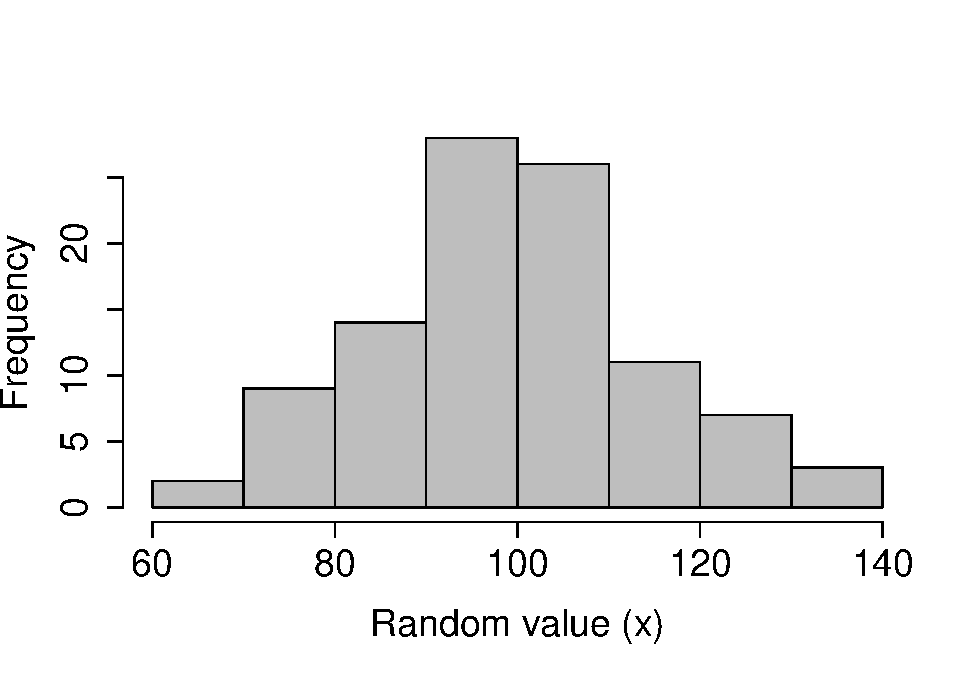
\includegraphics{_main_files/figure-latex/unnamed-chunk-5-1.pdf}

\subsection*{Sampling from a list of values}\label{sampling-from-a-list-of-values}
\addcontentsline{toc}{subsection}{Sampling from a list of values}

\begin{Shaded}
\begin{Highlighting}[]
\CommentTok{\# Example 1: sample randomly from the values 1:7}
\NormalTok{f }\OtherTok{\textless{}{-}} \FunctionTok{data.frame}\NormalTok{(}
  \AttributeTok{ID =} \FunctionTok{c}\NormalTok{(}\DecValTok{1}\SpecialCharTok{:}\DecValTok{100}\NormalTok{),}
  \AttributeTok{Score =} \FunctionTok{sample}\NormalTok{(}\AttributeTok{x=}\FunctionTok{c}\NormalTok{(}\DecValTok{1}\SpecialCharTok{:}\DecValTok{7}\NormalTok{),}\AttributeTok{size=}\DecValTok{100}\NormalTok{,}\AttributeTok{replace =} \ConstantTok{TRUE}\NormalTok{)}
\NormalTok{)}


\CommentTok{\# Example 2: set the probabilities for the possible responses}
\NormalTok{Prob\_info }\OtherTok{\textless{}{-}} \FunctionTok{c}\NormalTok{(}\FloatTok{0.02}\NormalTok{, }\FloatTok{0.03}\NormalTok{, }\FloatTok{0.05}\NormalTok{, }\FloatTok{0.1}\NormalTok{, }\FloatTok{0.1}\NormalTok{, }\FloatTok{0.4}\NormalTok{, }\FloatTok{0.4}\NormalTok{)}

\NormalTok{g }\OtherTok{\textless{}{-}} \FunctionTok{data.frame}\NormalTok{(}
  \AttributeTok{ID =} \FunctionTok{c}\NormalTok{(}\DecValTok{1}\SpecialCharTok{:}\DecValTok{100}\NormalTok{),}
  \AttributeTok{Score =} \FunctionTok{sample}\NormalTok{(}\AttributeTok{x=}\FunctionTok{c}\NormalTok{(}\DecValTok{1}\SpecialCharTok{:}\DecValTok{7}\NormalTok{),}\AttributeTok{size=}\DecValTok{100}\NormalTok{,}\AttributeTok{replace =} \ConstantTok{TRUE}\NormalTok{,}\AttributeTok{prob =}\NormalTok{ Prob\_info) }\CommentTok{\# use prob info}
\NormalTok{)}

\FunctionTok{hist}\NormalTok{(g}\SpecialCharTok{$}\NormalTok{Score, }\AttributeTok{xlab =} \StringTok{"Random value (x)"}\NormalTok{, }\AttributeTok{col =} \StringTok{"grey"}\NormalTok{, }\AttributeTok{main =} \StringTok{""}\NormalTok{, }\AttributeTok{cex.lab =} \FloatTok{1.5}\NormalTok{, }\AttributeTok{cex.axis =} \FloatTok{1.5}\NormalTok{)}
\end{Highlighting}
\end{Shaded}

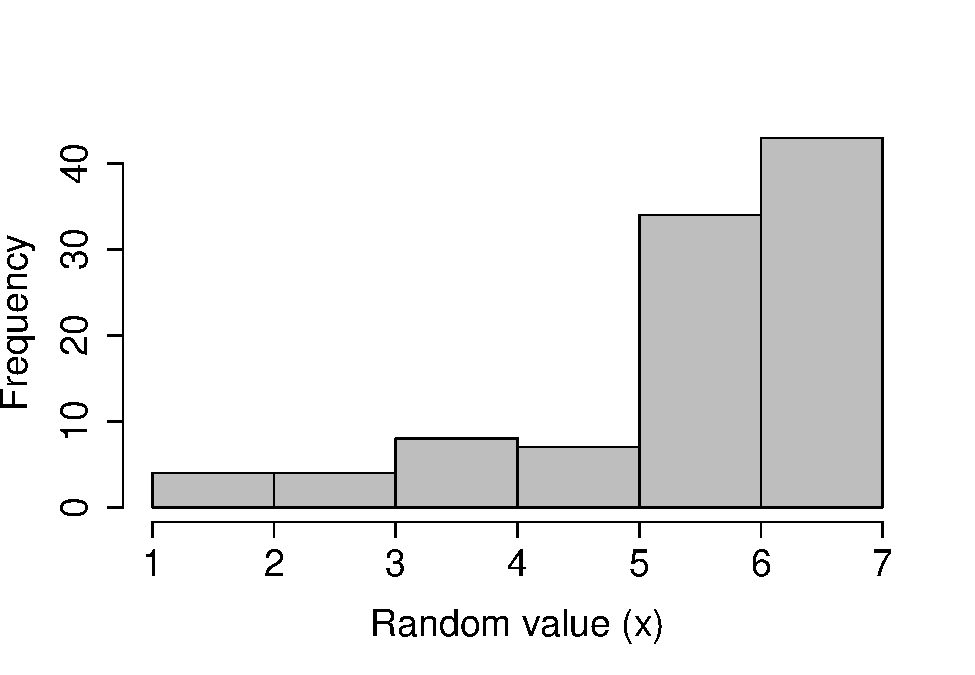
\includegraphics{_main_files/figure-latex/unnamed-chunk-6-1.pdf}

\subsection*{Example of a complete dataset}\label{example-of-a-complete-dataset}
\addcontentsline{toc}{subsection}{Example of a complete dataset}

\begin{Shaded}
\begin{Highlighting}[]
\CommentTok{\# Make data for a ctl group}
\NormalTok{Control\_group }\OtherTok{\textless{}{-}} \FunctionTok{data.frame}\NormalTok{(}
  \AttributeTok{ID =} \FunctionTok{c}\NormalTok{(}\DecValTok{1}\SpecialCharTok{:}\DecValTok{100}\NormalTok{),}
  \AttributeTok{Condition =} \StringTok{"Placebo"}\NormalTok{,}
  \AttributeTok{Baseline\_IQ =} \FunctionTok{rnorm}\NormalTok{(}\AttributeTok{n=}\DecValTok{100}\NormalTok{,}\AttributeTok{mean=}\DecValTok{100}\NormalTok{,}\AttributeTok{sd=}\DecValTok{15}\NormalTok{),}
  \AttributeTok{Post\_IQ =} \FunctionTok{rnorm}\NormalTok{(}\AttributeTok{n=}\DecValTok{100}\NormalTok{,}\AttributeTok{mean=}\DecValTok{100}\NormalTok{,}\AttributeTok{sd=}\DecValTok{15}\NormalTok{)}
\NormalTok{)}

\CommentTok{\# And experimental data with the exact same column headers}
\NormalTok{Experimental\_group }\OtherTok{\textless{}{-}} \FunctionTok{data.frame}\NormalTok{(}
  \AttributeTok{ID =} \FunctionTok{c}\NormalTok{(}\DecValTok{101}\SpecialCharTok{:}\DecValTok{200}\NormalTok{),}
  \AttributeTok{Condition =} \StringTok{"Drug"}\NormalTok{,}
  \AttributeTok{Baseline\_IQ =} \FunctionTok{rnorm}\NormalTok{(}\AttributeTok{n=}\DecValTok{100}\NormalTok{,}\AttributeTok{mean=}\DecValTok{100}\NormalTok{,}\AttributeTok{sd=}\DecValTok{15}\NormalTok{),}
  \AttributeTok{Post\_IQ =} \FunctionTok{rnorm}\NormalTok{(}\AttributeTok{n=}\DecValTok{100}\NormalTok{,}\AttributeTok{mean=}\DecValTok{130}\NormalTok{,}\AttributeTok{sd=}\DecValTok{15}\NormalTok{)}
\NormalTok{)}

\CommentTok{\# attach them together}
\NormalTok{JLB\_data }\OtherTok{\textless{}{-}} \FunctionTok{rbind}\NormalTok{(Control\_group,Experimental\_group)}
\end{Highlighting}
\end{Shaded}

\subsection*{Aggregate table of data}\label{aggregate-table-of-data}
\addcontentsline{toc}{subsection}{Aggregate table of data}

\begin{Shaded}
\begin{Highlighting}[]
\CommentTok{\# step 1 install packages }
\DocumentationTok{\#\# Do once per computer}

\CommentTok{\# install.packages(c("tidyverse","reshape2"))}

\CommentTok{\# Call the packages }
\DocumentationTok{\#\# Do this every session}

\FunctionTok{library}\NormalTok{(tidyverse) }\CommentTok{\# Call the tidyverse}
\FunctionTok{library}\NormalTok{(reshape2) }\CommentTok{\# Call reshape2 (for the "melt" function)}
\end{Highlighting}
\end{Shaded}

\begin{Shaded}
\begin{Highlighting}[]
\CommentTok{\# An example of "tidy text" (from the tidyverse):}
\NormalTok{table }\OtherTok{\textless{}{-}}\NormalTok{ JLB\_data }\SpecialCharTok{\%\textgreater{}\%} \CommentTok{\# Take the data AND THEN}
  \FunctionTok{melt}\NormalTok{(}\AttributeTok{id.vars =} \FunctionTok{c}\NormalTok{(}\StringTok{"ID"}\NormalTok{,}\StringTok{"Condition"}\NormalTok{)) }\SpecialCharTok{\%\textgreater{}\%} \CommentTok{\# Switch to long form AND THEN}
  \FunctionTok{group\_by}\NormalTok{(Condition,variable) }\SpecialCharTok{\%\textgreater{}\%} \CommentTok{\# Group by the IVs}
  \FunctionTok{summarise}\NormalTok{( }\CommentTok{\# Calculate descriptive stats}
    \AttributeTok{n =} \FunctionTok{n}\NormalTok{(),}
    \AttributeTok{mean =} \FunctionTok{mean}\NormalTok{(value),}
    \AttributeTok{sd =} \FunctionTok{sd}\NormalTok{(value),}
    \AttributeTok{min =} \FunctionTok{min}\NormalTok{(value),}
    \AttributeTok{max =} \FunctionTok{max}\NormalTok{(value)}
\NormalTok{  ) }\SpecialCharTok{\%\textgreater{}\%} \FunctionTok{mutate}\NormalTok{(}\AttributeTok{se =}\NormalTok{ sd }\SpecialCharTok{/} \FunctionTok{sqrt}\NormalTok{(n)) }\CommentTok{\# Create a column for SE, and compute it}

\CommentTok{\# Rename the columns for a better looking table}
\FunctionTok{colnames}\NormalTok{(table) }\OtherTok{\textless{}{-}} \FunctionTok{c}\NormalTok{(}\StringTok{"Condition"}\NormalTok{,}\StringTok{"Timepoint"}\NormalTok{,}\StringTok{"n"}\NormalTok{,}\StringTok{"mean"}\NormalTok{,}\StringTok{"sd"}\NormalTok{,}\StringTok{"min"}\NormalTok{,}\StringTok{"max"}\NormalTok{,}\StringTok{"se"}\NormalTok{)}

\CommentTok{\# a regular table}
\NormalTok{table}
\end{Highlighting}
\end{Shaded}

\begin{verbatim}
## # A tibble: 4 x 8
## # Groups:   Condition [2]
##   Condition Timepoint       n  mean    sd   min   max    se
##   <chr>     <fct>       <int> <dbl> <dbl> <dbl> <dbl> <dbl>
## 1 Drug      Baseline_IQ   100  96.8  13.9  63.1  137.  1.39
## 2 Drug      Post_IQ       100 131.   14.7  84.3  176.  1.47
## 3 Placebo   Baseline_IQ   100  99.3  14.5  67.9  137.  1.45
## 4 Placebo   Post_IQ       100  98.9  15.8  54.4  136.  1.58
\end{verbatim}

\begin{Shaded}
\begin{Highlighting}[]
\CommentTok{\# a pretty table }
\NormalTok{knitr}\SpecialCharTok{::}\FunctionTok{kable}\NormalTok{(table)}
\end{Highlighting}
\end{Shaded}

\begin{tabular}{l|l|r|r|r|r|r|r}
\hline
Condition & Timepoint & n & mean & sd & min & max & se\\
\hline
Drug & Baseline\_IQ & 100 & 96.79806 & 13.87755 & 63.13986 & 136.5700 & 1.387755\\
\hline
Drug & Post\_IQ & 100 & 131.05099 & 14.66883 & 84.29550 & 175.8569 & 1.466883\\
\hline
Placebo & Baseline\_IQ & 100 & 99.33318 & 14.50270 & 67.89372 & 136.8935 & 1.450270\\
\hline
Placebo & Post\_IQ & 100 & 98.91235 & 15.79230 & 54.43327 & 135.5055 & 1.579230\\
\hline
\end{tabular}

\emph{Please submit a single document for practical \#4. A .docx file is the preferred format.}

\chapter{Correlation Statistics and Plots}\label{correlation-statistics-and-plots}

\section*{1. Thinking About Association}\label{thinking-about-association}
\addcontentsline{toc}{section}{1. Thinking About Association}

As part of your final paper, you will be proposing an association between your dependent variable (DV) and a covariate of interest. In the last practical assignment, you developed some `priors' around what the DV and covariate would look like. In this assignment, you will be asked to justify, simulate, and report the association between your DV and your covariate.

The first step is to \textbf{write an introductory paragraph} that reminds us what your proposed DV and covariate are, and why you believe they should be associated. You can cite papers later- first just explain how you think the two variables work together. For example, if the your DV were ``feelings of stress'' and your covariate were ``optimism'', tell us a bit about the relationship between them from a theoretical perspective- do optimistic people tend not to perceive stressful life events the same way? Perhaps optimistic people just don't experience the same level of physiological reaction to stressors and see the world a less threatening place? Help us understand why you think these variables ought to be related, or at least why it is possible that they are.

\section*{2. What is already known about these varaibles?}\label{what-is-already-known-about-these-varaibles}
\addcontentsline{toc}{section}{2. What is already known about these varaibles?}

\textbf{Write a paragraph or two describing what we know about your proposed DV and covariate}. What direction are the proposed associations? In this section, you should cite at least 2 empirical, peer-reviewed papers that help you to estimate the expected association size, using APA format (minus hanging indents) and including the full references below the paragraph(s).

Most importantly, we need to get specific about the expect association value. In your brief literature review, please report any measure of association, which will often be a correlation (r) or beta estimate (b), along with some interpretation of the effect size involved. Effect sizes can be described by specific effect size statistics like cohen's d or partial eta2, or they could be describe by confidence intervals.

If you cannot find any reports of correlation values in the literature, then you will have to argue from theory about your predicted effect size:

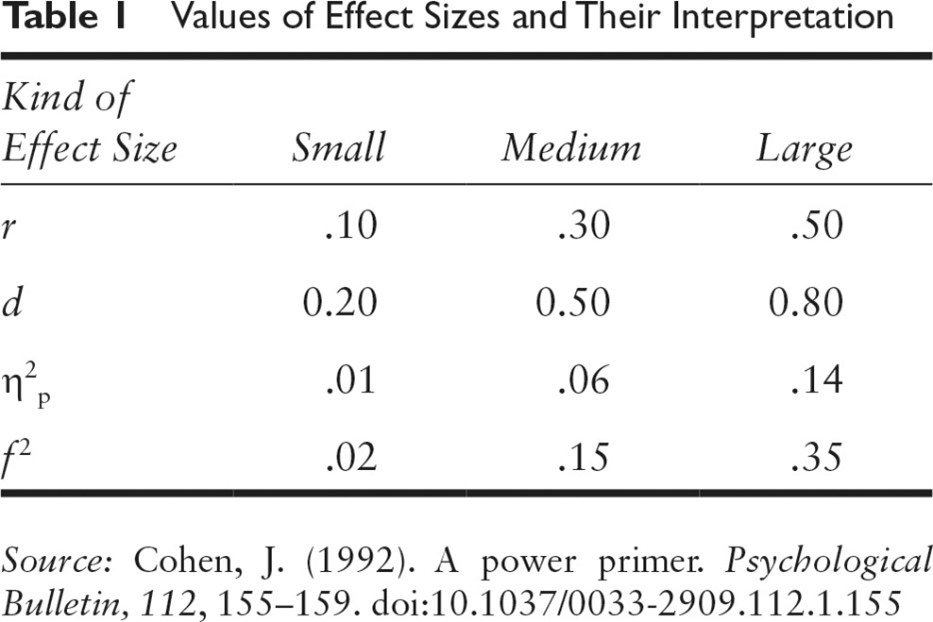
\includegraphics{Figs/effect_size.jpg}

Please note that finding correlations \textgreater.30 (or \textless{} -.30) is rare in a lot of psychology (especially human research; animal studies tend to yield larger effect sizes), so you will need to justify the effect size you expect to find.

\section*{3. Power Analysis: what sample size should you use?}\label{power-analysis-what-sample-size-should-you-use}
\addcontentsline{toc}{section}{3. Power Analysis: what sample size should you use?}

\textbf{\emph{For this portion of the assignment, make sure that you have your code blocks set to \texttt{echo\ =\ TRUE,\ message\ =\ FALSE,\ warning\ =\ FALSE}.}} This will print the code and the result, but not excessive the messages that R sends.

Use an online calculator (link in Lecture\_5 slides to my favorite one, but there are many available) to estimate the sample size needed given the estimated correlation that you derived from your literature search.

\section*{4. A picture is worth 100 words\ldots{}}\label{a-picture-is-worth-100-words}
\addcontentsline{toc}{section}{4. A picture is worth 100 words\ldots{}}

\textbf{Simulate} two columns of data to represent your DV and covariate. Use the sample size that you determined was required for adequate power.

\textbf{Generate} a ggplot (scatterplot) of the data with a linear line of best fit. You can format this graph in any way that you see fit. Feel free to be creative! Every element of this chart can be tweaked to your specifications. Feel free to \texttt{Google} how to change specific aesthetics.

\textbf{Save} the ggplot as a high-quality .png image (\texttt{dpi\ =\ 300}), and call back the high quality image for your assignment. Add a figure caption to describe the relationship that you have depicted in the chart.

\textbf{Call back} the image that you saved to showcase your simulated data in pictoral form!

\section*{5. Reflect}\label{reflect-3}
\addcontentsline{toc}{section}{5. Reflect}

Write a closing paragraph (3-5 sentences) summarizing what it is like trying to estimate an association / correlation from the literature. What did you think about creating your first data visualization using R? Were you surprised by the number of participants required to detect your effect with 80\% power? Feeling confused about any of these concepts? Is there anything that would have improved your experience doing this assignment?

\section*{Code for Practical \#4}\label{code-for-practical-4}
\addcontentsline{toc}{section}{Code for Practical \#4}

\begin{Shaded}
\begin{Highlighting}[]
\CommentTok{\# Set up how the code chunks will print}
\NormalTok{knitr}\SpecialCharTok{::}\NormalTok{opts\_chunk}\SpecialCharTok{$}\FunctionTok{set}\NormalTok{(}\AttributeTok{echo =} \ConstantTok{TRUE}\NormalTok{, }\CommentTok{\# Show the code}
                      \AttributeTok{warning =} \ConstantTok{FALSE}\NormalTok{, }\CommentTok{\# Hide the warnings}
                      \AttributeTok{message =} \ConstantTok{FALSE}\NormalTok{) }\CommentTok{\# Hide the messages}
\end{Highlighting}
\end{Shaded}

\subsection*{Generate Data}\label{generate-data}
\addcontentsline{toc}{subsection}{Generate Data}

\begin{Shaded}
\begin{Highlighting}[]
\CommentTok{\# You must install packages before you can use them.}
\CommentTok{\# You only needd to install once per computer. }

\CommentTok{\# install.packages(c("faux","tidyverse")) \# Remove leading hashtag to run this line! }


\CommentTok{\# Once the packages are installed, you can load them to your current R session using the library() command }

\FunctionTok{library}\NormalTok{(faux)}
\FunctionTok{library}\NormalTok{(tidyverse)}

\CommentTok{\# Set a consistent start point for "random" data generation}
\CommentTok{\# Makes it so the output will be consistent}

\FunctionTok{set.seed}\NormalTok{(}\DecValTok{123}\NormalTok{) }\CommentTok{\# Can be any value. }


\CommentTok{\# Generate data. Specify the number of rows, number of variables, means for the columns, sd\textquotesingle{}s for the columns, and the correlation between the columns.}

\NormalTok{data }\OtherTok{\textless{}{-}} \FunctionTok{rnorm\_multi}\NormalTok{(}\AttributeTok{n =} \DecValTok{85}\NormalTok{, }\AttributeTok{vars =} \DecValTok{2}\NormalTok{, }\AttributeTok{mu =} \FunctionTok{c}\NormalTok{(}\DecValTok{65}\NormalTok{,}\DecValTok{100}\NormalTok{), }\AttributeTok{sd =} \FunctionTok{c}\NormalTok{(}\DecValTok{10}\NormalTok{,}\DecValTok{15}\NormalTok{), }\AttributeTok{r =} \SpecialCharTok{{-}}\FloatTok{0.3}\NormalTok{)}
\end{Highlighting}
\end{Shaded}

\subsection*{Check out the data}\label{check-out-the-data}
\addcontentsline{toc}{subsection}{Check out the data}

\begin{Shaded}
\begin{Highlighting}[]
\CommentTok{\# Show me the first 6 rows of data: }
\FunctionTok{head}\NormalTok{(data)}
\end{Highlighting}
\end{Shaded}

\begin{verbatim}
##         X1        X2
## 1 64.74322  90.80306
## 2 56.44198  93.49663
## 3 53.76554 121.72313
## 4 67.53304 101.96359
## 5 54.27693  98.64371
## 6 48.10980 122.44146
\end{verbatim}

\begin{Shaded}
\begin{Highlighting}[]
\CommentTok{\# Rename the columns to represent your variables }
\FunctionTok{colnames}\NormalTok{(data) }\OtherTok{\textless{}{-}} \FunctionTok{c}\NormalTok{(}\StringTok{"Age"}\NormalTok{,}\StringTok{"IQ"}\NormalTok{)}
\end{Highlighting}
\end{Shaded}

\subsection*{Check the correlation}\label{check-the-correlation}
\addcontentsline{toc}{subsection}{Check the correlation}

\begin{Shaded}
\begin{Highlighting}[]
\CommentTok{\# Check the correlation between the two columns }
\CommentTok{\# If you don\textquotesingle{}t like it, play around with the value in set.seed until you are happy. }
\FunctionTok{cor.test}\NormalTok{(data}\SpecialCharTok{$}\NormalTok{Age,data}\SpecialCharTok{$}\NormalTok{IQ)}
\end{Highlighting}
\end{Shaded}

\begin{verbatim}
## 
##  Pearson's product-moment correlation
## 
## data:  data$Age and data$IQ
## t = -2.5503, df = 83, p-value = 0.0126
## alternative hypothesis: true correlation is not equal to 0
## 95 percent confidence interval:
##  -0.45646873 -0.05988606
## sample estimates:
##        cor 
## -0.2695696
\end{verbatim}

\subsection*{Code to generate a basic scatterplot:}\label{code-to-generate-a-basic-scatterplot}
\addcontentsline{toc}{subsection}{Code to generate a basic scatterplot:}

\begin{Shaded}
\begin{Highlighting}[]
\NormalTok{data }\SpecialCharTok{\%\textgreater{}\%}
  \FunctionTok{ggplot}\NormalTok{(}\FunctionTok{aes}\NormalTok{(}\AttributeTok{x =}\NormalTok{ Age, }\AttributeTok{y =}\NormalTok{ IQ))}\SpecialCharTok{+}
  \FunctionTok{geom\_point}\NormalTok{()}\SpecialCharTok{+}
  \FunctionTok{geom\_smooth}\NormalTok{(}\AttributeTok{method =} \StringTok{"lm"}\NormalTok{)}
\end{Highlighting}
\end{Shaded}

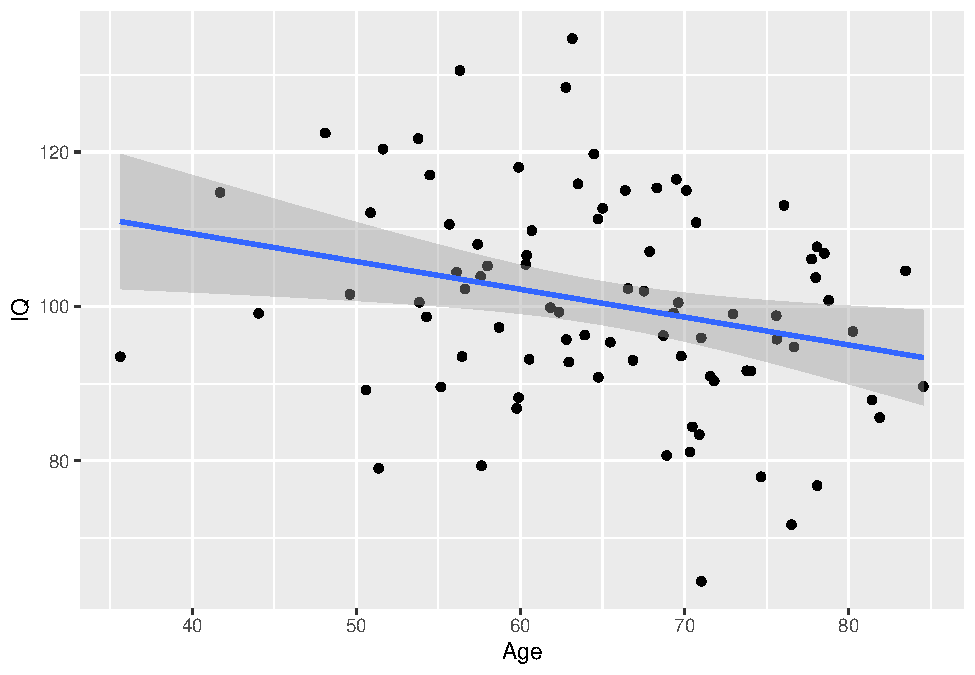
\includegraphics{_main_files/figure-latex/unnamed-chunk-15-1.pdf}

\subsection*{A fancier, better looking scatterplot:}\label{a-fancier-better-looking-scatterplot}
\addcontentsline{toc}{subsection}{A fancier, better looking scatterplot:}

\begin{Shaded}
\begin{Highlighting}[]
\NormalTok{a }\OtherTok{\textless{}{-}}\NormalTok{ data }\SpecialCharTok{\%\textgreater{}\%}
  \FunctionTok{ggplot}\NormalTok{(}\FunctionTok{aes}\NormalTok{(}\AttributeTok{x =}\NormalTok{ Age, }\AttributeTok{y =}\NormalTok{ IQ))}\SpecialCharTok{+}
  \FunctionTok{geom\_point}\NormalTok{(}\AttributeTok{size =} \DecValTok{4}\NormalTok{, }\AttributeTok{alpha =} \FloatTok{0.5}\NormalTok{, }\AttributeTok{colour =} \StringTok{"\#800020"}\NormalTok{)}\SpecialCharTok{+}
  \FunctionTok{geom\_smooth}\NormalTok{(}\AttributeTok{method =} \StringTok{"lm"}\NormalTok{, }\AttributeTok{colour=}\StringTok{"\#800020"}\NormalTok{, }\AttributeTok{fill=}\StringTok{"\#800020"}\NormalTok{)}\SpecialCharTok{+}
  \FunctionTok{theme\_classic}\NormalTok{()}\SpecialCharTok{+}
  \FunctionTok{theme}\NormalTok{(}\AttributeTok{plot.title =} \FunctionTok{element\_text}\NormalTok{(}\AttributeTok{hjust=}\FloatTok{0.5}\NormalTok{))}\SpecialCharTok{+}
  \FunctionTok{labs}\NormalTok{(}
    \AttributeTok{x =} \StringTok{"Age of Participants"}\NormalTok{,}
    \AttributeTok{y =} \StringTok{"IQ Score"}\NormalTok{,}
    \AttributeTok{title =} \StringTok{"Relationship Between Age and IQ"}
\NormalTok{  )}\SpecialCharTok{+}
  \FunctionTok{xlim}\NormalTok{(}\DecValTok{30}\NormalTok{,}\DecValTok{90}\NormalTok{)}\SpecialCharTok{+}
  \FunctionTok{ylim}\NormalTok{(}\DecValTok{60}\NormalTok{,}\DecValTok{140}\NormalTok{)}

\CommentTok{\# Save the chart once you\textquotesingle{}re happy with it as a high quality .png image}
\FunctionTok{ggsave}\NormalTok{(}\StringTok{"JLB\_graph.png"}\NormalTok{,a,}\AttributeTok{height=}\DecValTok{4}\NormalTok{,}\AttributeTok{width=}\DecValTok{4}\NormalTok{,}\AttributeTok{dpi =} \DecValTok{300}\NormalTok{)}

\CommentTok{\# Add in the high quality image saved above }
\NormalTok{knitr}\SpecialCharTok{::}\FunctionTok{include\_graphics}\NormalTok{(}\StringTok{"JLB\_graph.png"}\NormalTok{)}
\end{Highlighting}
\end{Shaded}

\begin{figure}
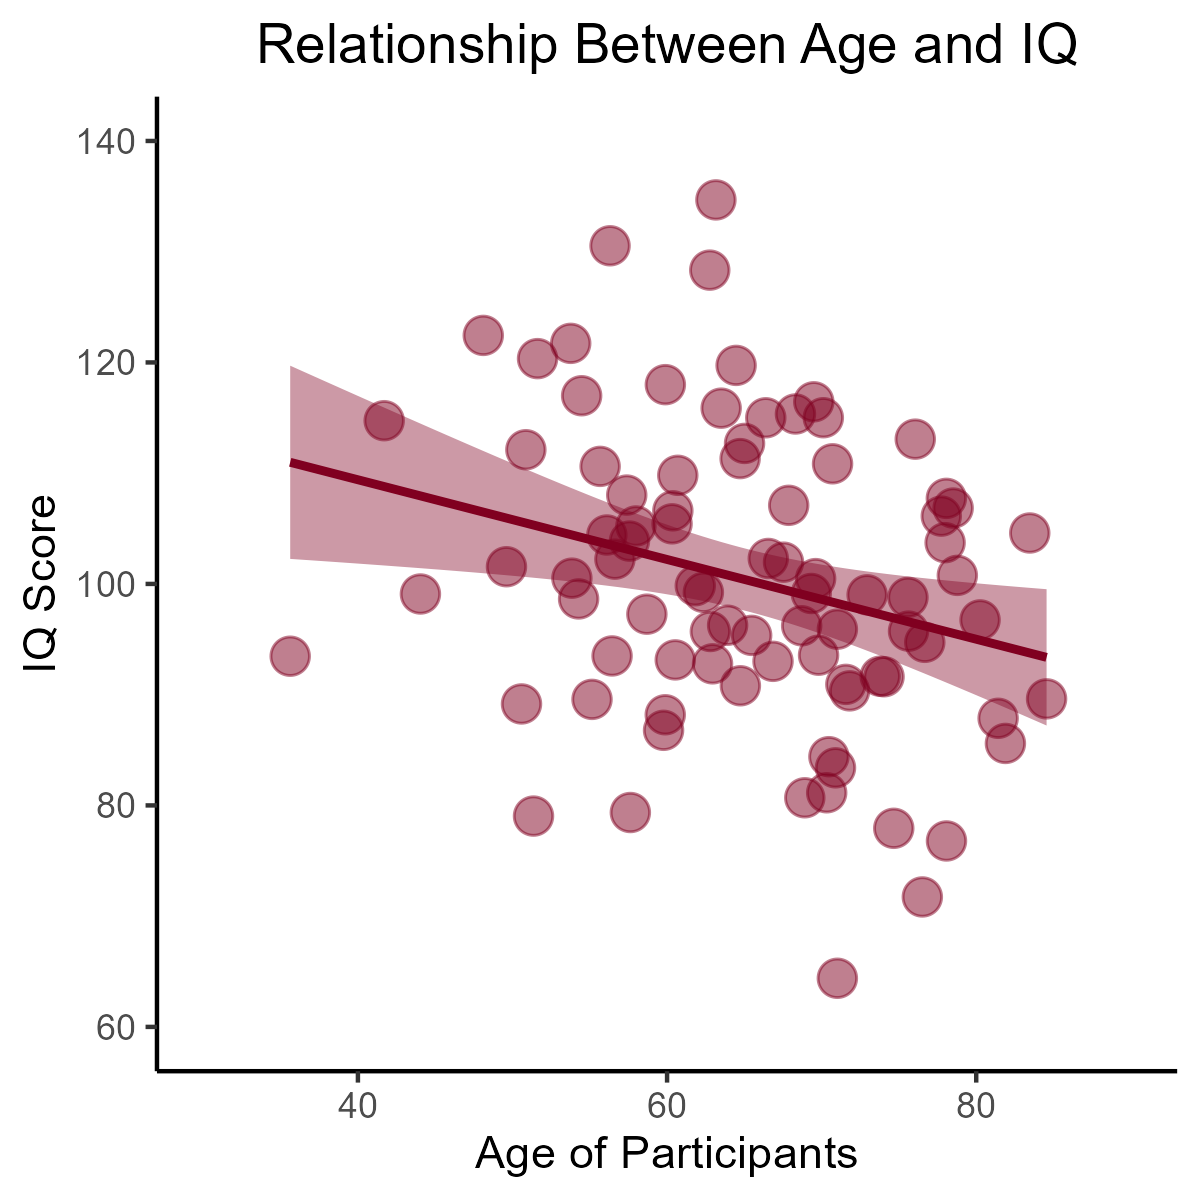
\includegraphics[width=16.67in]{JLB_graph} \caption{ADD A FIGURE CAPTION HERE}\label{fig:unnamed-chunk-16}
\end{figure}

\chapter{Connecting the IV and Covariate}\label{connecting-the-iv-and-covariate}

\section*{1. Thinking About Causality}\label{thinking-about-causality}
\addcontentsline{toc}{section}{1. Thinking About Causality}

\textbf{Strength of association} is a necessary step in determining whether there is a causal relationship between X and Y, but it is not sufficient for inferring causality. For your final assignment, you will be designing an experiment that involves at least 2 independent variables (The ``IV'' and the ``covariate'' that you have explored in the previous assignments).

In prior assignments, you were already asked to provide a simple group comparison or manipulation (an IV) that could reveal a difference in your DV. Now, please \textbf{write a paragraph explaining this decision in more detail} - what is the theory or explanation for why this manipulation works?

\section*{2. What is already known?}\label{what-is-already-known}
\addcontentsline{toc}{section}{2. What is already known?}

The second step is getting back into literature review. \textbf{Write a paragraph or two} in APA format describing what we know about your proposed manipulation and DV. What in the research literature (citing 2-3 papers) makes you believe that this manipulation will influence your DV? What direction is the proposed effect, i.e., does the manipulation increase or decrease your DV.

Most importantly, we need to get specific about the expected change in the DV when you manipulate the IV. In your brief literature review, please report any measure of effect size, which will often be a cohen's d or partial eta-squared (η2) or beta estimate (b). Best of all would be to see how much of a change in the DV in units of the DV the manipulation makes.

\section*{3. Connect the theory of the IV-DV relationship to your proposed covariate.}\label{connect-the-theory-of-the-iv-dv-relationship-to-your-proposed-covariate.}
\addcontentsline{toc}{section}{3. Connect the theory of the IV-DV relationship to your proposed covariate.}

Explain how the continuous covariate might modulate the relationship between the IV and DV that you are proposing. Use literature to support your ideas. Be very clear about the proposed direction of the effects. Would you expect the IV to affect all levels of the covariate equally? Why or why not?

Reference at least one article that suggests a relationship between your \textbf{independent variable} and \textbf{proposed covariate} to support your narrative.

\section*{4. Transform the continuous covariate to a categorical variable}\label{transform-the-continuous-covariate-to-a-categorical-variable}
\addcontentsline{toc}{section}{4. Transform the continuous covariate to a categorical variable}

Using the r-code that you developed in practical 4, have a look at your continuous covariate and continuous DV. Imagine that this continuous relationship represents the real-world construct. If you were to divide this continuum into categories, how many would you use and why? Explain why it might make sense to use this number of categories (either from a statistical or a theoretical perspective).

Back to the code! Using the data that you simulated in practical 4, transform the continuous covariate into a new column that is categorical. Use ggplot to make a bar chart with error bars that represent the standard error of the mean and individual points to represent your theoretical participants' scores on the DV. Use the method that we learned in practical 4 to save off a high quality .png image of this chart, then call it back using knitr::kable().

Compute a statistical analysis to measure whether the categories that you selected differ significantly from one another on your DV. This analysis should either be a two-sample t-test or a one-way ANOVA (depending on the number of categories you chose). Interpret the analysis using an APA statement.

Make sure that you have \texttt{echo\ =\ TURE,\ warning\ =\ FALSE,\ message\ =\ FALSE} set for your code blocks so that R will print out your code and the results, but will hide messages and warnings.

\section*{5. Reflect}\label{reflect-4}
\addcontentsline{toc}{section}{5. Reflect}

What are the advantageous and disadvantages to transforming the continuous covariate into a categorical variable? Was it difficult to choose the number of categories to divide your covariate into? What did you think about generating a bar chart through ggplot? How did running your first statistical analysis through R go? Is there anything that would have helped you learn these processes more effectively? Any lingering questions?

\section*{Code for Practical \#5}\label{code-for-practical-5}
\addcontentsline{toc}{section}{Code for Practical \#5}

\begin{Shaded}
\begin{Highlighting}[]
\CommentTok{\# Set up how the code chunks will print}
\NormalTok{knitr}\SpecialCharTok{::}\NormalTok{opts\_chunk}\SpecialCharTok{$}\FunctionTok{set}\NormalTok{(}\AttributeTok{echo =} \ConstantTok{TRUE}\NormalTok{, }\CommentTok{\# Show the code}
                      \AttributeTok{warning =} \ConstantTok{FALSE}\NormalTok{, }\CommentTok{\# Hide the warnings}
                      \AttributeTok{message =} \ConstantTok{FALSE}\NormalTok{) }\CommentTok{\# Hide the messages}

\FunctionTok{library}\NormalTok{(faux)}
\FunctionTok{library}\NormalTok{(tidyverse)}
\end{Highlighting}
\end{Shaded}

\subsection*{Generate data}\label{generate-data-1}
\addcontentsline{toc}{subsection}{Generate data}

The block of code below is the same as what was computed in practical \#4. Here, the theory is to generate two columns of data of a given n (i.e., number of rows) with an approximate correlation between the columns specified. The two columns should represent your chosen covariate and dependent variable.

\begin{Shaded}
\begin{Highlighting}[]
\CommentTok{\# Set a consistent start point for "random" data generation}
\CommentTok{\# Makes it so the output will be consistent}

\FunctionTok{set.seed}\NormalTok{(}\DecValTok{123}\NormalTok{) }\CommentTok{\# Can be any value. }

\CommentTok{\# Generate data. Specify the number of rows, number of variables, means for the columns, sd\textquotesingle{}s for the columns, and the correlation between the columns.}

\NormalTok{data }\OtherTok{\textless{}{-}} \FunctionTok{rnorm\_multi}\NormalTok{(}\AttributeTok{n =} \DecValTok{85}\NormalTok{, }\AttributeTok{vars =} \DecValTok{2}\NormalTok{, }\AttributeTok{mu =} \FunctionTok{c}\NormalTok{(}\DecValTok{65}\NormalTok{,}\DecValTok{100}\NormalTok{), }\AttributeTok{sd =} \FunctionTok{c}\NormalTok{(}\DecValTok{10}\NormalTok{,}\DecValTok{15}\NormalTok{), }\AttributeTok{r =} \SpecialCharTok{{-}}\FloatTok{0.3}\NormalTok{)}

\CommentTok{\# Rename the columns to represent your variables }
\FunctionTok{colnames}\NormalTok{(data) }\OtherTok{\textless{}{-}} \FunctionTok{c}\NormalTok{(}\StringTok{"Age"}\NormalTok{,}\StringTok{"IQ"}\NormalTok{)}

\DocumentationTok{\#\#\#\#\#\# Everything above this point is copy \& pasted from practical \#4. }
\end{Highlighting}
\end{Shaded}

\subsection*{Transform}\label{transform}
\addcontentsline{toc}{subsection}{Transform}

Generate a 3rd column of data that will represent a categorized version of the covariate. Divite the participants into categories based on specified cut points.

\begin{Shaded}
\begin{Highlighting}[]
\CommentTok{\# Transform the continuous variable into categories}
\NormalTok{data}\SpecialCharTok{$}\NormalTok{age\_cat }\OtherTok{\textless{}{-}} \FunctionTok{cut}\NormalTok{(data}\SpecialCharTok{$}\NormalTok{Age,}
                    \AttributeTok{breaks =} \FunctionTok{c}\NormalTok{(}\SpecialCharTok{{-}}\ConstantTok{Inf}\NormalTok{, }\DecValTok{65}\NormalTok{, }\ConstantTok{Inf}\NormalTok{), }\CommentTok{\# cut points}
                    \AttributeTok{labels =} \FunctionTok{c}\NormalTok{(}\StringTok{"Under 65"}\NormalTok{, }\StringTok{"Over 65"}\NormalTok{)) }\CommentTok{\# labels}

\FunctionTok{head}\NormalTok{(data) }\CommentTok{\# Check out the data frame with the new column}
\end{Highlighting}
\end{Shaded}

\begin{verbatim}
##        Age        IQ  age_cat
## 1 64.74322  90.80306 Under 65
## 2 56.44198  93.49663 Under 65
## 3 53.76554 121.72313 Under 65
## 4 67.53304 101.96359  Over 65
## 5 54.27693  98.64371 Under 65
## 6 48.10980 122.44146 Under 65
\end{verbatim}

\subsection*{Make a Bar Graph}\label{make-a-bar-graph}
\addcontentsline{toc}{subsection}{Make a Bar Graph}

\begin{Shaded}
\begin{Highlighting}[]
\CommentTok{\# A bar graph}
\NormalTok{a }\OtherTok{\textless{}{-}}\NormalTok{ data }\SpecialCharTok{\%\textgreater{}\%}
  \FunctionTok{group\_by}\NormalTok{(age\_cat) }\SpecialCharTok{\%\textgreater{}\%}
  \FunctionTok{summarise}\NormalTok{(}
    \AttributeTok{n=}\FunctionTok{n}\NormalTok{(),}
    \AttributeTok{mean=}\FunctionTok{mean}\NormalTok{(IQ),}
    \AttributeTok{sd=}\FunctionTok{sd}\NormalTok{(IQ)}
\NormalTok{  ) }\SpecialCharTok{\%\textgreater{}\%} \FunctionTok{mutate}\NormalTok{(}\AttributeTok{se=}\NormalTok{sd }\SpecialCharTok{/} \FunctionTok{sqrt}\NormalTok{(n)) }\SpecialCharTok{\%\textgreater{}\%}
  \FunctionTok{ggplot}\NormalTok{(}\FunctionTok{aes}\NormalTok{(}\AttributeTok{x=}\NormalTok{age\_cat,}\AttributeTok{y=}\NormalTok{mean, }\AttributeTok{colour =}\NormalTok{ age\_cat, }\AttributeTok{fill=}\NormalTok{ age\_cat, }\AttributeTok{shape=}\NormalTok{age\_cat)) }\SpecialCharTok{+}
  \FunctionTok{geom\_bar}\NormalTok{(}\AttributeTok{stat=}\StringTok{"identity"}\NormalTok{,}\AttributeTok{alpha=}\FloatTok{0.2}\NormalTok{)}\SpecialCharTok{+}
  \FunctionTok{geom\_errorbar}\NormalTok{(}\FunctionTok{aes}\NormalTok{(}\AttributeTok{x=}\NormalTok{age\_cat,}\AttributeTok{ymin=}\NormalTok{mean}\SpecialCharTok{{-}}\NormalTok{se,}\AttributeTok{ymax=}\NormalTok{mean}\SpecialCharTok{+}\NormalTok{se),}\AttributeTok{width=}\FloatTok{0.5}\NormalTok{)}\SpecialCharTok{+}
  \FunctionTok{geom\_jitter}\NormalTok{(}\AttributeTok{data =}\NormalTok{ data,}\FunctionTok{aes}\NormalTok{(}\AttributeTok{x=}\NormalTok{age\_cat,}\AttributeTok{y=}\NormalTok{IQ),}\AttributeTok{height=}\DecValTok{0}\NormalTok{, }\AttributeTok{width=}\FloatTok{0.25}\NormalTok{, }\AttributeTok{size=}\DecValTok{3}\NormalTok{,}\AttributeTok{alpha=}\FloatTok{0.5}\NormalTok{)}\SpecialCharTok{+}
  \FunctionTok{scale\_colour\_manual}\NormalTok{(}\AttributeTok{values =} \FunctionTok{c}\NormalTok{(}\StringTok{"grey"}\NormalTok{,}\StringTok{"black"}\NormalTok{))}\SpecialCharTok{+}
  \FunctionTok{scale\_fill\_manual}\NormalTok{(}\AttributeTok{values=}\FunctionTok{c}\NormalTok{(}\StringTok{"grey"}\NormalTok{,}\StringTok{"black"}\NormalTok{))}\SpecialCharTok{+}
  \FunctionTok{theme\_classic}\NormalTok{()}\SpecialCharTok{+}
  \FunctionTok{theme}\NormalTok{(}\AttributeTok{legend.position =} \StringTok{"none"}\NormalTok{)}\SpecialCharTok{+}
  \FunctionTok{theme}\NormalTok{(}\AttributeTok{plot.title =} \FunctionTok{element\_text}\NormalTok{(}\AttributeTok{hjust=}\FloatTok{0.5}\NormalTok{))}\SpecialCharTok{+}
  \FunctionTok{labs}\NormalTok{(}
    \AttributeTok{x=}\StringTok{"Age Categories"}\NormalTok{,}
    \AttributeTok{y=}\StringTok{"IQ Score"}\NormalTok{,}
    \AttributeTok{title=}\StringTok{"Effect of Age on }\SpecialCharTok{\textbackslash{}n}\StringTok{ IQ Scores"}
\NormalTok{  )}

\FunctionTok{ggsave}\NormalTok{(}\StringTok{"2\_bars.png"}\NormalTok{,a,}\AttributeTok{height=}\DecValTok{4}\NormalTok{,}\AttributeTok{width=}\DecValTok{3}\NormalTok{,}\AttributeTok{dpi=}\DecValTok{300}\NormalTok{)}

\NormalTok{knitr}\SpecialCharTok{::}\FunctionTok{include\_graphics}\NormalTok{(}\StringTok{"2\_bars.png"}\NormalTok{)}
\end{Highlighting}
\end{Shaded}

\begin{figure}
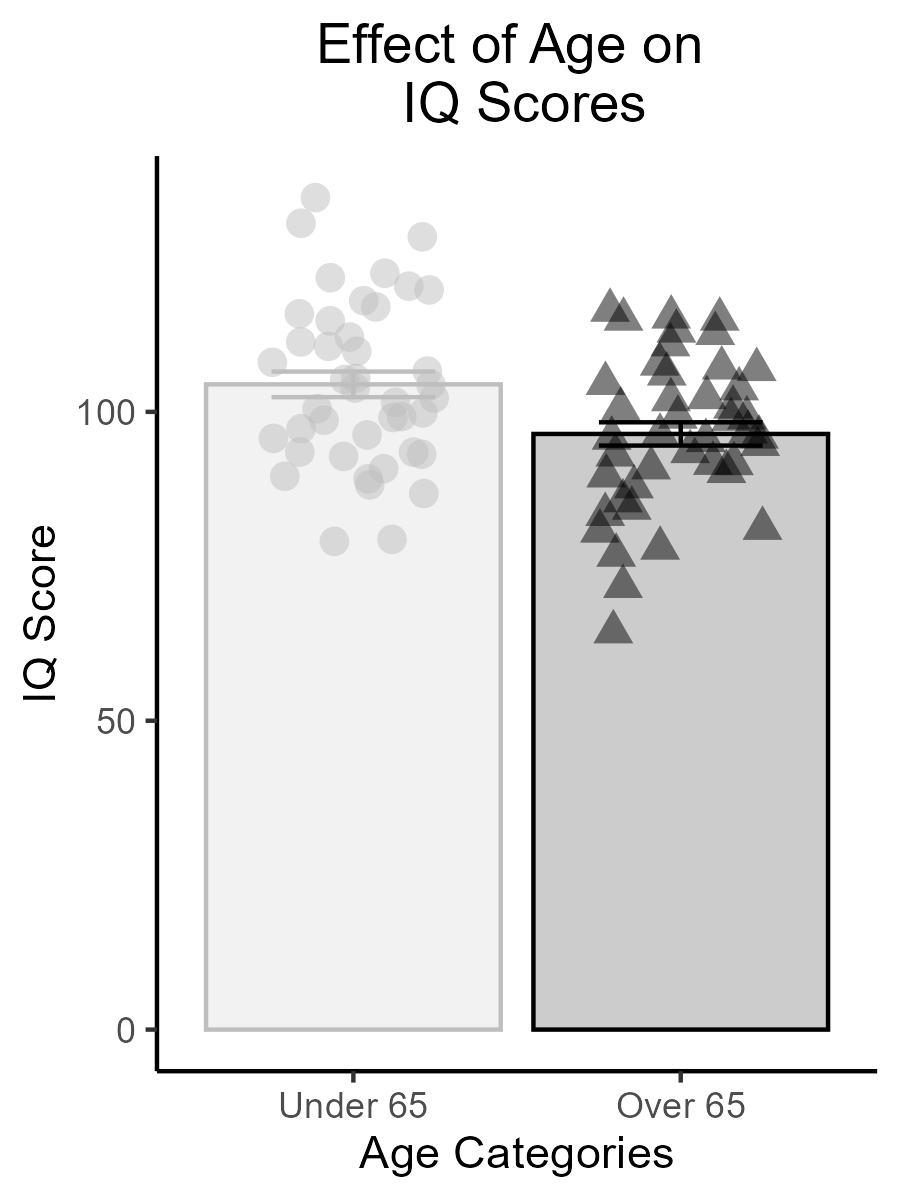
\includegraphics[width=12.5in]{2_bars} \caption{First example: Here, I divided the continuous covariate into two categories.}\label{fig:unnamed-chunk-20}
\end{figure}

\subsection*{Analyze}\label{analyze}
\addcontentsline{toc}{subsection}{Analyze}

Run a t-test because there are only two groups here.

\begin{Shaded}
\begin{Highlighting}[]
\CommentTok{\# Levigne\textquotesingle{}s test for equity of variances}
\FunctionTok{var.test}\NormalTok{(}\AttributeTok{data =}\NormalTok{ data, IQ }\SpecialCharTok{\textasciitilde{}}\NormalTok{ age\_cat)}
\end{Highlighting}
\end{Shaded}

\begin{verbatim}
## 
##  F test to compare two variances
## 
## data:  IQ by age_cat
## F = 1.1772, num df = 41, denom df = 42, p-value = 0.6007
## alternative hypothesis: true ratio of variances is not equal to 1
## 95 percent confidence interval:
##  0.6359244 2.1842525
## sample estimates:
## ratio of variances 
##           1.177203
\end{verbatim}

\begin{Shaded}
\begin{Highlighting}[]
\CommentTok{\# A t.test when variances are not unequal}
\FunctionTok{t.test}\NormalTok{(}\AttributeTok{data =}\NormalTok{ data, IQ }\SpecialCharTok{\textasciitilde{}}\NormalTok{ age\_cat, }\AttributeTok{var.equal =} \ConstantTok{TRUE}\NormalTok{)}
\end{Highlighting}
\end{Shaded}

\begin{verbatim}
## 
##  Two Sample t-test
## 
## data:  IQ by age_cat
## t = 2.8695, df = 83, p-value = 0.005214
## alternative hypothesis: true difference in means between group Under 65 and group Over 65 is not equal to 0
## 95 percent confidence interval:
##   2.462339 13.586680
## sample estimates:
## mean in group Under 65  mean in group Over 65 
##              104.45180               96.42729
\end{verbatim}

\subsection*{3-category exmaple}\label{category-exmaple}
\addcontentsline{toc}{subsection}{3-category exmaple}

\begin{Shaded}
\begin{Highlighting}[]
\CommentTok{\# An example of how to divide the continuous variable into 3 categories}
\NormalTok{data}\SpecialCharTok{$}\NormalTok{age\_cat }\OtherTok{\textless{}{-}} \FunctionTok{cut}\NormalTok{(data}\SpecialCharTok{$}\NormalTok{Age,}
                    \AttributeTok{breaks =} \FunctionTok{c}\NormalTok{(}\SpecialCharTok{{-}}\ConstantTok{Inf}\NormalTok{, }\DecValTok{60}\NormalTok{, }\DecValTok{70}\NormalTok{, }\ConstantTok{Inf}\NormalTok{),}
                    \AttributeTok{labels =} \FunctionTok{c}\NormalTok{(}\StringTok{"Under 60"}\NormalTok{,}\StringTok{"60{-}70"}\NormalTok{, }\StringTok{"Over 70"}\NormalTok{))}

\CommentTok{\# Graph for the 3{-}category data }
\DocumentationTok{\#\# Only change vs above is the number of coulours! (Robust!!)}
\NormalTok{JLB\_garph }\OtherTok{\textless{}{-}}\NormalTok{ data }\SpecialCharTok{\%\textgreater{}\%} \CommentTok{\# Assign the chart to an object}
  \FunctionTok{group\_by}\NormalTok{(age\_cat) }\SpecialCharTok{\%\textgreater{}\%}
  \FunctionTok{summarise}\NormalTok{(}
    \AttributeTok{n=}\FunctionTok{n}\NormalTok{(),}
    \AttributeTok{mean=}\FunctionTok{mean}\NormalTok{(IQ),}
    \AttributeTok{sd=}\FunctionTok{sd}\NormalTok{(IQ)}
\NormalTok{  ) }\SpecialCharTok{\%\textgreater{}\%} \FunctionTok{mutate}\NormalTok{(}\AttributeTok{se=}\NormalTok{sd }\SpecialCharTok{/} \FunctionTok{sqrt}\NormalTok{(n)) }\SpecialCharTok{\%\textgreater{}\%}
  \FunctionTok{ggplot}\NormalTok{(}\FunctionTok{aes}\NormalTok{(}\AttributeTok{x=}\NormalTok{age\_cat,}\AttributeTok{y=}\NormalTok{mean, }\AttributeTok{colour =}\NormalTok{ age\_cat, }\AttributeTok{fill=}\NormalTok{ age\_cat, }\AttributeTok{shape=}\NormalTok{age\_cat)) }\SpecialCharTok{+}
  \FunctionTok{geom\_bar}\NormalTok{(}\AttributeTok{stat=}\StringTok{"identity"}\NormalTok{,}\AttributeTok{alpha=}\FloatTok{0.2}\NormalTok{)}\SpecialCharTok{+}
  \FunctionTok{geom\_errorbar}\NormalTok{(}\FunctionTok{aes}\NormalTok{(}\AttributeTok{x=}\NormalTok{age\_cat,}\AttributeTok{ymin=}\NormalTok{mean}\SpecialCharTok{{-}}\NormalTok{se,}\AttributeTok{ymax=}\NormalTok{mean}\SpecialCharTok{+}\NormalTok{se),}\AttributeTok{width=}\FloatTok{0.5}\NormalTok{)}\SpecialCharTok{+}
  \FunctionTok{geom\_jitter}\NormalTok{(}\AttributeTok{data =}\NormalTok{ data,}\FunctionTok{aes}\NormalTok{(}\AttributeTok{x=}\NormalTok{age\_cat,}\AttributeTok{y=}\NormalTok{IQ),}\AttributeTok{height=}\DecValTok{0}\NormalTok{, }\AttributeTok{width=}\FloatTok{0.25}\NormalTok{, }\AttributeTok{size=}\DecValTok{3}\NormalTok{,}\AttributeTok{alpha=}\FloatTok{0.5}\NormalTok{)}\SpecialCharTok{+}
  \FunctionTok{scale\_colour\_manual}\NormalTok{(}\AttributeTok{values =} \FunctionTok{c}\NormalTok{(}\StringTok{"grey"}\NormalTok{,}\StringTok{"black"}\NormalTok{,}\StringTok{"blue"}\NormalTok{))}\SpecialCharTok{+}
  \FunctionTok{scale\_fill\_manual}\NormalTok{(}\AttributeTok{values=}\FunctionTok{c}\NormalTok{(}\StringTok{"grey"}\NormalTok{,}\StringTok{"black"}\NormalTok{,}\StringTok{"blue"}\NormalTok{))}\SpecialCharTok{+}
  \FunctionTok{theme\_classic}\NormalTok{()}\SpecialCharTok{+}
  \FunctionTok{theme}\NormalTok{(}\AttributeTok{legend.position =} \StringTok{"none"}\NormalTok{)}\SpecialCharTok{+}
  \FunctionTok{theme}\NormalTok{(}\AttributeTok{plot.title =} \FunctionTok{element\_text}\NormalTok{(}\AttributeTok{hjust=}\FloatTok{0.5}\NormalTok{))}\SpecialCharTok{+}
  \FunctionTok{labs}\NormalTok{(}
    \AttributeTok{x=}\StringTok{"Age Categories"}\NormalTok{,}
    \AttributeTok{y=}\StringTok{"IQ Score"}\NormalTok{,}
    \AttributeTok{title=}\StringTok{"Effect of Age on }\SpecialCharTok{\textbackslash{}n}\StringTok{ IQ Scores"}
\NormalTok{  )}

\CommentTok{\# Save a high quality .png copy of the image}
\FunctionTok{ggsave}\NormalTok{(}\StringTok{"JLB\_prc\_5.png"}\NormalTok{,JLB\_garph,}\AttributeTok{height=}\DecValTok{4}\NormalTok{,}\AttributeTok{width=}\DecValTok{4}\NormalTok{,}\AttributeTok{dpi=}\DecValTok{300}\NormalTok{)}

\CommentTok{\# Call back the high quality image}
\NormalTok{knitr}\SpecialCharTok{::}\FunctionTok{include\_graphics}\NormalTok{(}\StringTok{"JLB\_prc\_5.png"}\NormalTok{)}
\end{Highlighting}
\end{Shaded}

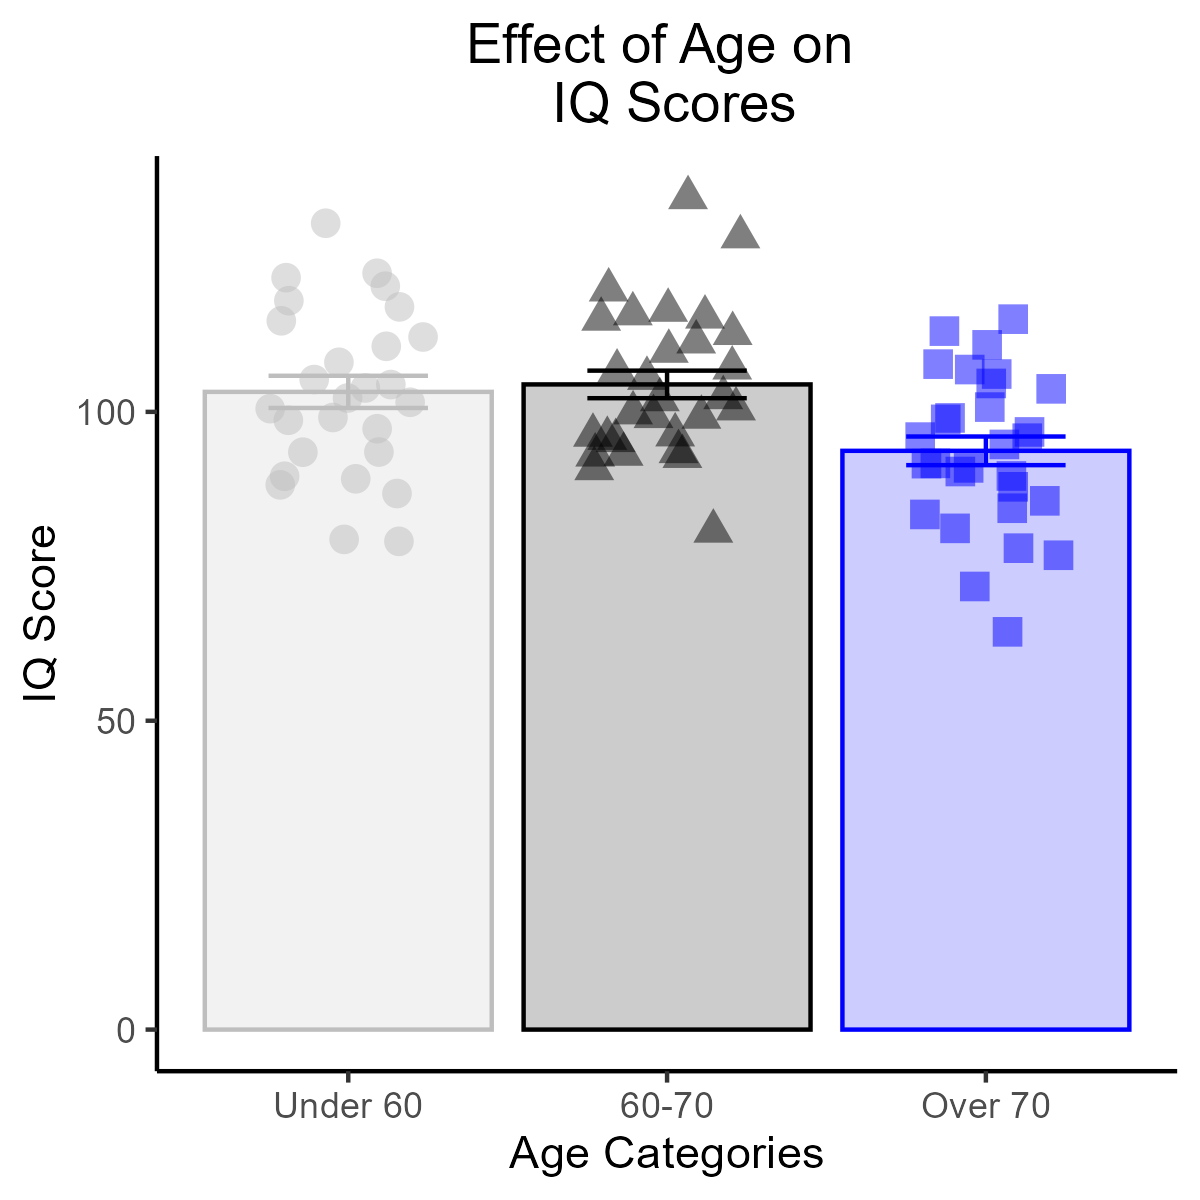
\includegraphics[width=16.67in]{JLB_prc_5}

\subsection{Analyze 3-category example}\label{analyze-3-category-example}

When there are more than two groups, use ANOVA instead of a t-test. If the results from the omnibus test of significance indicate p \textless{} 0.05, run Tukey's honestly significant difference test to figure out \emph{where} the group differences are.

\begin{Shaded}
\begin{Highlighting}[]
\CommentTok{\# Run a one{-}way ANOVA}
\NormalTok{res }\OtherTok{\textless{}{-}} \FunctionTok{aov}\NormalTok{(}\AttributeTok{data =}\NormalTok{ data, IQ }\SpecialCharTok{\textasciitilde{}}\NormalTok{ age\_cat)}
\FunctionTok{summary}\NormalTok{(res)}
\end{Highlighting}
\end{Shaded}

\begin{verbatim}
##             Df Sum Sq Mean Sq F value  Pr(>F)   
## age_cat      2   1996   998.2   6.218 0.00306 **
## Residuals   82  13163   160.5                   
## ---
## Signif. codes:  0 '***' 0.001 '**' 0.01 '*' 0.05 '.' 0.1 ' ' 1
\end{verbatim}

\begin{Shaded}
\begin{Highlighting}[]
\CommentTok{\# Follow up to find out which groups differ from one{-}another. }
\FunctionTok{TukeyHSD}\NormalTok{(res)}
\end{Highlighting}
\end{Shaded}

\begin{verbatim}
##   Tukey multiple comparisons of means
##     95% family-wise confidence level
## 
## Fit: aov(formula = IQ ~ age_cat, data = data)
## 
## $age_cat
##                        diff        lwr       upr     p adj
## 60-70-Under 60     1.205088  -6.882959  9.293134 0.9327115
## Over 70-Under 60  -9.545689 -17.633735 -1.457642 0.0165397
## Over 70-60-70    -10.750776 -18.693080 -2.808472 0.0050015
\end{verbatim}

\chapter*{Capstone Project: A Simulated Research Paper}\label{capstone-project-a-simulated-research-paper}
\addcontentsline{toc}{chapter}{Capstone Project: A Simulated Research Paper}

\section*{Overview}\label{overview-1}
\addcontentsline{toc}{section}{Overview}

The purpose of the practical assignments that you have completed across the term was to provide you with all of the tools needed to execute a fictitious experiment. Now, you will integrate these skills to produce your final written assignment.

The final assignment should demonstrate your understanding of research methodology, document generation using Rstudio and competency using R code. The goal of this project should be to produce an output document that you could present as a ``portfolio piece'' in an academic (or other) context.

For this reason, please \textbf{show code used to generate analyses} as well as the results from those analyses. \textbf{Hide code used to generate figures}, but show the results (aka the high-quality images). Please submit a single .docx file that was generated through Rmarkdwon as your submission.

\section*{Introduction}\label{introduction}
\addcontentsline{toc}{section}{Introduction}

The expected length of the introduction section is \textasciitilde{} 1000 words. Make sure that you divide your ideas into paragraphs that each discuss a unique component of your study. The introduction section should be at least 5 paragraphs long, and should not be more than 10 paragraphs. We do not typically use subheading within the introduction section of an empirical article. You should introduce the articles that you have sourced throughout the practical assignments by describing \textbf{what's been done}, \textbf{what's been found}, and \textbf{what these findings means}. Use the past literature to provide rationale for the experiment that you are currently conducting.

In the final paragraph of the introduction section, you should explain the purpose of your paper (e.g., describe how you will be extending upon the findings that you've summarized so far). Make sure that you clearly explain all of the variables you will be using: The independent variable, the dependent variable, and the covariate.

\section*{Methods}\label{methods}
\addcontentsline{toc}{section}{Methods}

Divide your methods into ``participants'', ``materials'', ``procedure'', ``statistical analyses'' (or similar) subheadings. Explain transparently that you will be simulating data using Rstudio to demonstrate the theoretical study that you have designed. Describe the method for determining your sample size and the final number of participants you will simulate. Provide descriptions of the methods and procedure so that an new reader that is knowledgeable about experimental design and Rstudio would be able to recreate your simulated experiment exactly.

\begin{Shaded}
\begin{Highlighting}[]
\DocumentationTok{\#\#\# Use code from Practical 4: }

\CommentTok{\# Set a consistent start point for "random" data generation}
\CommentTok{\# Makes it so the output will be consistent}

\FunctionTok{set.seed}\NormalTok{(}\DecValTok{123}\NormalTok{) }\CommentTok{\# Can be any value. }

\CommentTok{\# Generate data. Specify the number of rows, number of variables, means for the columns, sd\textquotesingle{}s for the columns, and the correlation between the columns.}

\NormalTok{data }\OtherTok{\textless{}{-}} \FunctionTok{rnorm\_multi}\NormalTok{(}\AttributeTok{n =} \DecValTok{85}\NormalTok{, }\AttributeTok{vars =} \DecValTok{2}\NormalTok{, }\AttributeTok{mu =} \FunctionTok{c}\NormalTok{(}\DecValTok{65}\NormalTok{,}\DecValTok{100}\NormalTok{), }\AttributeTok{sd =} \FunctionTok{c}\NormalTok{(}\DecValTok{10}\NormalTok{,}\DecValTok{15}\NormalTok{), }\AttributeTok{r =} \SpecialCharTok{{-}}\FloatTok{0.3}\NormalTok{)}

\CommentTok{\# Rename the columns to represent your variables }
\FunctionTok{colnames}\NormalTok{(data) }\OtherTok{\textless{}{-}} \FunctionTok{c}\NormalTok{(}\StringTok{"Age"}\NormalTok{,}\StringTok{"IQ"}\NormalTok{)}
\FunctionTok{head}\NormalTok{(data)}
\end{Highlighting}
\end{Shaded}

\begin{verbatim}
##        Age        IQ
## 1 64.74322  90.80306
## 2 56.44198  93.49663
## 3 53.76554 121.72313
## 4 67.53304 101.96359
## 5 54.27693  98.64371
## 6 48.10980 122.44146
\end{verbatim}

\emph{Do not worry about the length of your methods or results section, just take the space that you need to fully describe your experimental proceedings / findings.}

\section*{Results}\label{results}
\addcontentsline{toc}{section}{Results}

Divide your results section into subheadings that describe different statistical analyses. The results of the analyses should be printed in both versions of your submission. Center your figures and provide figure captions. Make sure that each figure has a label (e.g., Figure 1), and that each of the figures is referenced in-text.

Think about keeping your analysis strategy \textbf{succinct} and \textbf{logical}. You need to balance volume with importance - show you understanding of data storytelling by presenting the analyses clearly using simple, direct sentences. Think about the reader - make your series of outputs \textbf{\emph{as easy to follow as possible}}.

\subsection*{Correlation Analysis}\label{correlation-analysis}
\addcontentsline{toc}{subsection}{Correlation Analysis}

Analyze, interpret, discuss, and plot the continuous relationship between the covariate and the dependent variable (practical \#4).

\begin{Shaded}
\begin{Highlighting}[]
\FunctionTok{cor.test}\NormalTok{(data}\SpecialCharTok{$}\NormalTok{Age,data}\SpecialCharTok{$}\NormalTok{IQ)}
\end{Highlighting}
\end{Shaded}

\begin{verbatim}
## 
##  Pearson's product-moment correlation
## 
## data:  data$Age and data$IQ
## t = -2.5503, df = 83, p-value = 0.0126
## alternative hypothesis: true correlation is not equal to 0
## 95 percent confidence interval:
##  -0.45646873 -0.05988606
## sample estimates:
##        cor 
## -0.2695696
\end{verbatim}

\subsection*{One-Way Analysis}\label{one-way-analysis}
\addcontentsline{toc}{subsection}{One-Way Analysis}

Explain, perform, graph, analyze, and interpret the transformation of the continuous covariate to a categorical variable (practical \#5). Make sure that you are clear about the number of levels that you are using, and the rationale for this choice. Test whether there is a ``basal'' difference between the groups using the appropriate analysis (t-test or ANOVA) and interpret the results.

\begin{Shaded}
\begin{Highlighting}[]
\CommentTok{\# Transform the continuous variable into categories}
\NormalTok{data}\SpecialCharTok{$}\NormalTok{age\_cat }\OtherTok{\textless{}{-}} \FunctionTok{cut}\NormalTok{(data}\SpecialCharTok{$}\NormalTok{Age,}
                    \AttributeTok{breaks =} \FunctionTok{c}\NormalTok{(}\SpecialCharTok{{-}}\ConstantTok{Inf}\NormalTok{, }\DecValTok{65}\NormalTok{, }\ConstantTok{Inf}\NormalTok{), }\CommentTok{\# cut points}
                    \AttributeTok{labels =} \FunctionTok{c}\NormalTok{(}\StringTok{"Under 65"}\NormalTok{, }\StringTok{"Over 65"}\NormalTok{)) }\CommentTok{\# labels}
\FunctionTok{head}\NormalTok{(data)}
\end{Highlighting}
\end{Shaded}

\begin{verbatim}
##        Age        IQ  age_cat
## 1 64.74322  90.80306 Under 65
## 2 56.44198  93.49663 Under 65
## 3 53.76554 121.72313 Under 65
## 4 67.53304 101.96359  Over 65
## 5 54.27693  98.64371 Under 65
## 6 48.10980 122.44146 Under 65
\end{verbatim}

\begin{Shaded}
\begin{Highlighting}[]
\CommentTok{\# Levigne\textquotesingle{}s test for equity of variances}
\FunctionTok{var.test}\NormalTok{(}\AttributeTok{data =}\NormalTok{ data, IQ }\SpecialCharTok{\textasciitilde{}}\NormalTok{ age\_cat)}
\end{Highlighting}
\end{Shaded}

\begin{verbatim}
## 
##  F test to compare two variances
## 
## data:  IQ by age_cat
## F = 1.1772, num df = 41, denom df = 42, p-value = 0.6007
## alternative hypothesis: true ratio of variances is not equal to 1
## 95 percent confidence interval:
##  0.6359244 2.1842525
## sample estimates:
## ratio of variances 
##           1.177203
\end{verbatim}

\begin{Shaded}
\begin{Highlighting}[]
\CommentTok{\# A t.test when variances are not unequal}
\FunctionTok{t.test}\NormalTok{(}\AttributeTok{data =}\NormalTok{ data, IQ }\SpecialCharTok{\textasciitilde{}}\NormalTok{ age\_cat, }\AttributeTok{var.equal =} \ConstantTok{TRUE}\NormalTok{)}
\end{Highlighting}
\end{Shaded}

\begin{verbatim}
## 
##  Two Sample t-test
## 
## data:  IQ by age_cat
## t = 2.8695, df = 83, p-value = 0.005214
## alternative hypothesis: true difference in means between group Under 65 and group Over 65 is not equal to 0
## 95 percent confidence interval:
##   2.462339 13.586680
## sample estimates:
## mean in group Under 65  mean in group Over 65 
##              104.45180               96.42729
\end{verbatim}

\subsection*{Factorial ANOVA}\label{factorial-anova}
\addcontentsline{toc}{subsection}{Factorial ANOVA}

Compute, interpret, and graph the results of the factorial ANOVA. Make sure that you run ALL of the appropriate follow-up comparisons, and explain what the results of each analysis means. You can graph the same data multiple ways if that helps tell the story of the various comparisons. Each project will look different - focus on conveying your data in the way that makes the most sense given your design.

\begin{Shaded}
\begin{Highlighting}[]
\DocumentationTok{\#\# Generate Final Dataset: }

\FunctionTok{set.seed}\NormalTok{(}\DecValTok{426}\NormalTok{)}

\CommentTok{\# Split your data frame into data frames corresponding to your levels of the categorized covaritae: }

\NormalTok{Under\_65 }\OtherTok{\textless{}{-}}\NormalTok{ data[data}\SpecialCharTok{$}\NormalTok{age\_cat }\SpecialCharTok{==} \StringTok{"Under 65"}\NormalTok{, ]}
\NormalTok{Over\_65 }\OtherTok{\textless{}{-}}\NormalTok{ data[data}\SpecialCharTok{$}\NormalTok{age\_cat }\SpecialCharTok{==} \StringTok{"Over 65"}\NormalTok{, ]}

\CommentTok{\# Randomly assign your independent variable to half the members of each group: }

\NormalTok{Under\_65}\SpecialCharTok{$}\NormalTok{Drug }\OtherTok{\textless{}{-}} \FunctionTok{c}\NormalTok{(}\FunctionTok{rep}\NormalTok{(}\StringTok{"Control"}\NormalTok{,}\DecValTok{21}\NormalTok{), }\FunctionTok{rep}\NormalTok{(}\StringTok{"Drug"}\NormalTok{,}\DecValTok{21}\NormalTok{))}
\NormalTok{Over\_65}\SpecialCharTok{$}\NormalTok{Drug }\OtherTok{\textless{}{-}} \FunctionTok{c}\NormalTok{(}\FunctionTok{rep}\NormalTok{(}\StringTok{"Control"}\NormalTok{,}\DecValTok{21}\NormalTok{), }\FunctionTok{rep}\NormalTok{(}\StringTok{"Drug"}\NormalTok{,}\DecValTok{22}\NormalTok{))}

\CommentTok{\# Split the data frame by the experimental groups}

\NormalTok{Under\_65\_control }\OtherTok{\textless{}{-}}\NormalTok{ Under\_65[Under\_65}\SpecialCharTok{$}\NormalTok{Drug }\SpecialCharTok{==} \StringTok{"Control"}\NormalTok{, ]}
\NormalTok{Under\_65\_drug }\OtherTok{\textless{}{-}}\NormalTok{ Under\_65[Under\_65}\SpecialCharTok{$}\NormalTok{Drug }\SpecialCharTok{==} \StringTok{"Drug"}\NormalTok{, ]}

\NormalTok{Over\_65\_control }\OtherTok{\textless{}{-}}\NormalTok{ Over\_65[Over\_65}\SpecialCharTok{$}\NormalTok{Drug }\SpecialCharTok{==} \StringTok{"Control"}\NormalTok{, ]}
\NormalTok{Over\_65\_drug }\OtherTok{\textless{}{-}}\NormalTok{ Over\_65[Over\_65}\SpecialCharTok{$}\NormalTok{Drug }\SpecialCharTok{==} \StringTok{"Drug"}\NormalTok{, ]}

\CommentTok{\# Create distributions of the proposed outcome after "intervention" (application of the IV)}

\NormalTok{Under\_65\_control}\SpecialCharTok{$}\NormalTok{Post\_IQ }\OtherTok{\textless{}{-}} \FunctionTok{rnorm}\NormalTok{(}\AttributeTok{n =} \DecValTok{21}\NormalTok{, }\AttributeTok{mean =} \DecValTok{100}\NormalTok{, }\AttributeTok{sd =} \DecValTok{15}\NormalTok{)}
\NormalTok{Under\_65\_drug}\SpecialCharTok{$}\NormalTok{Post\_IQ }\OtherTok{\textless{}{-}} \FunctionTok{rnorm}\NormalTok{(}\AttributeTok{n =} \DecValTok{21}\NormalTok{, }\AttributeTok{mean =} \DecValTok{100}\NormalTok{, }\AttributeTok{sd =} \DecValTok{15}\NormalTok{)}

\NormalTok{Over\_65\_control}\SpecialCharTok{$}\NormalTok{Post\_IQ }\OtherTok{\textless{}{-}} \FunctionTok{rnorm}\NormalTok{(}\AttributeTok{n =} \DecValTok{21}\NormalTok{, }\AttributeTok{mean =} \DecValTok{90}\NormalTok{, }\AttributeTok{sd =} \DecValTok{10}\NormalTok{)}
\NormalTok{Over\_65\_drug}\SpecialCharTok{$}\NormalTok{Post\_IQ }\OtherTok{\textless{}{-}} \FunctionTok{rnorm}\NormalTok{(}\AttributeTok{n =} \DecValTok{22}\NormalTok{, }\AttributeTok{mean =} \DecValTok{100}\NormalTok{, }\AttributeTok{sd =} \DecValTok{15}\NormalTok{)}

\NormalTok{final\_data }\OtherTok{\textless{}{-}} \FunctionTok{rbind}\NormalTok{(Under\_65\_control,Under\_65\_drug,Over\_65\_control,Over\_65\_drug)}

\FunctionTok{head}\NormalTok{(final\_data)}
\end{Highlighting}
\end{Shaded}

\begin{verbatim}
##        Age        IQ  age_cat    Drug   Post_IQ
## 1 64.74322  90.80306 Under 65 Control 115.36923
## 2 56.44198  93.49663 Under 65 Control 131.36582
## 3 53.76554 121.72313 Under 65 Control 103.77843
## 5 54.27693  98.64371 Under 65 Control  95.39799
## 6 48.10980 122.44146 Under 65 Control 113.34786
## 7 57.98470 105.23238 Under 65 Control 116.07211
\end{verbatim}

\begin{Shaded}
\begin{Highlighting}[]
\CommentTok{\# Aggregate your final data to check it out: }
\NormalTok{knitr}\SpecialCharTok{::}\FunctionTok{kable}\NormalTok{(final\_data }\SpecialCharTok{\%\textgreater{}\%}
  \FunctionTok{group\_by}\NormalTok{(Drug,age\_cat) }\SpecialCharTok{\%\textgreater{}\%}
  \FunctionTok{summarise}\NormalTok{(}
    \AttributeTok{n=}\FunctionTok{n}\NormalTok{(),}
    \AttributeTok{mean=}\FunctionTok{mean}\NormalTok{(Post\_IQ),}
    \AttributeTok{sd=}\FunctionTok{sd}\NormalTok{(Post\_IQ)}
\NormalTok{  ) }\SpecialCharTok{\%\textgreater{}\%} \FunctionTok{mutate}\NormalTok{(}\AttributeTok{se =}\NormalTok{ sd }\SpecialCharTok{/} \FunctionTok{sqrt}\NormalTok{(n))}
\NormalTok{)}
\end{Highlighting}
\end{Shaded}

\begin{tabular}{l|l|r|r|r|r}
\hline
Drug & age\_cat & n & mean & sd & se\\
\hline
Control & Under 65 & 21 & 100.20596 & 14.62407 & 3.191234\\
\hline
Control & Over 65 & 21 & 88.54052 & 12.04785 & 2.629057\\
\hline
Drug & Under 65 & 21 & 101.12417 & 16.27543 & 3.551591\\
\hline
Drug & Over 65 & 22 & 106.40972 & 13.09813 & 2.792530\\
\hline
\end{tabular}

\begin{Shaded}
\begin{Highlighting}[]
\CommentTok{\# Switch to long{-}form}
\NormalTok{long\_data }\OtherTok{\textless{}{-}}\NormalTok{ final\_data }\SpecialCharTok{\%\textgreater{}\%} 
  \FunctionTok{mutate}\NormalTok{(}\AttributeTok{ID =} \FunctionTok{c}\NormalTok{(}\DecValTok{1}\SpecialCharTok{:}\DecValTok{85}\NormalTok{)) }\SpecialCharTok{\%\textgreater{}\%} \CommentTok{\# Add an ID column}
  \FunctionTok{melt}\NormalTok{(}\AttributeTok{id.vars=}\FunctionTok{c}\NormalTok{(}\StringTok{"ID"}\NormalTok{,}\StringTok{"Drug"}\NormalTok{,}\StringTok{"age\_cat"}\NormalTok{,}\StringTok{"Age"}\NormalTok{))}

\FunctionTok{head}\NormalTok{(long\_data)}
\end{Highlighting}
\end{Shaded}

\begin{verbatim}
##   ID    Drug  age_cat      Age variable     value
## 1  1 Control Under 65 64.74322       IQ  90.80306
## 2  2 Control Under 65 56.44198       IQ  93.49663
## 3  3 Control Under 65 53.76554       IQ 121.72313
## 4  4 Control Under 65 54.27693       IQ  98.64371
## 5  5 Control Under 65 48.10980       IQ 122.44146
## 6  6 Control Under 65 57.98470       IQ 105.23238
\end{verbatim}

\begin{Shaded}
\begin{Highlighting}[]
\CommentTok{\# I\textquotesingle{}m making 2 graphs to show the same data two ways}
\DocumentationTok{\#\# You choose one way that makes the most sense given your design.}
\NormalTok{A }\OtherTok{\textless{}{-}}\NormalTok{ long\_data }\SpecialCharTok{\%\textgreater{}\%}
  \FunctionTok{group\_by}\NormalTok{(age\_cat,Drug,variable) }\SpecialCharTok{\%\textgreater{}\%}
  \FunctionTok{summarise}\NormalTok{(}
    \AttributeTok{n=}\FunctionTok{n}\NormalTok{(),}
    \AttributeTok{mean=}\FunctionTok{mean}\NormalTok{(value),}
    \AttributeTok{sd=}\FunctionTok{sd}\NormalTok{(value)}
\NormalTok{  ) }\SpecialCharTok{\%\textgreater{}\%} \FunctionTok{mutate}\NormalTok{(}\AttributeTok{se =}\NormalTok{ sd }\SpecialCharTok{/}\FunctionTok{sqrt}\NormalTok{(n)) }\SpecialCharTok{\%\textgreater{}\%}
  \FunctionTok{ggplot}\NormalTok{(}\FunctionTok{aes}\NormalTok{(}\AttributeTok{x=}\NormalTok{variable,}\AttributeTok{y=}\NormalTok{mean,}\AttributeTok{colour=}\NormalTok{age\_cat,}\AttributeTok{shape=}\NormalTok{age\_cat,}\AttributeTok{group=}\NormalTok{age\_cat))}\SpecialCharTok{+}
  \FunctionTok{geom\_point}\NormalTok{(}\AttributeTok{size=}\DecValTok{4}\NormalTok{,}\AttributeTok{alpha=}\FloatTok{0.5}\NormalTok{)}\SpecialCharTok{+}
  \FunctionTok{geom\_line}\NormalTok{(}\AttributeTok{linewidth=}\DecValTok{1}\NormalTok{, }\AttributeTok{alpha=}\FloatTok{0.5}\NormalTok{)}\SpecialCharTok{+}
  \FunctionTok{geom\_errorbar}\NormalTok{(}\FunctionTok{aes}\NormalTok{(}\AttributeTok{x=}\NormalTok{variable,}\AttributeTok{ymin=}\NormalTok{mean}\SpecialCharTok{{-}}\NormalTok{se,}\AttributeTok{ymax=}\NormalTok{mean}\SpecialCharTok{+}\NormalTok{se),}\AttributeTok{width=}\FloatTok{0.5}\NormalTok{)}\SpecialCharTok{+}
  \FunctionTok{geom\_jitter}\NormalTok{(}\AttributeTok{data =}\NormalTok{ long\_data,}\FunctionTok{aes}\NormalTok{(}\AttributeTok{x=}\NormalTok{variable,}\AttributeTok{y=}\NormalTok{value),}\AttributeTok{size=}\DecValTok{3}\NormalTok{,}\AttributeTok{alpha=}\FloatTok{0.2}\NormalTok{,}\AttributeTok{height=}\DecValTok{0}\NormalTok{,}\AttributeTok{width=}\FloatTok{0.25}\NormalTok{)}\SpecialCharTok{+}
  \FunctionTok{facet\_wrap}\NormalTok{(}\SpecialCharTok{\textasciitilde{}}\NormalTok{Drug)}\SpecialCharTok{+}
  \FunctionTok{theme\_classic}\NormalTok{()}\SpecialCharTok{+}
  \FunctionTok{theme}\NormalTok{(}\AttributeTok{legend.position =} \FunctionTok{c}\NormalTok{(}\DecValTok{0}\NormalTok{,}\DecValTok{1}\NormalTok{),}\AttributeTok{legend.justification =} \FunctionTok{c}\NormalTok{(}\DecValTok{0}\NormalTok{,}\DecValTok{1}\NormalTok{))}\SpecialCharTok{+}
  \FunctionTok{theme}\NormalTok{(}\AttributeTok{legend.background =} \FunctionTok{element\_rect}\NormalTok{(}\AttributeTok{fill=}\StringTok{"transparent"}\NormalTok{))}\SpecialCharTok{+}
  \FunctionTok{ylim}\NormalTok{(}\DecValTok{50}\NormalTok{,}\DecValTok{150}\NormalTok{)}\SpecialCharTok{+}
  \FunctionTok{labs}\NormalTok{(}
    \AttributeTok{x=}\StringTok{"Time of Testing"}\NormalTok{,}
    \AttributeTok{y=}\StringTok{"IQ Score"}
\NormalTok{  )}

\NormalTok{B }\OtherTok{\textless{}{-}}\NormalTok{ long\_data }\SpecialCharTok{\%\textgreater{}\%}
  \FunctionTok{group\_by}\NormalTok{(age\_cat,Drug,variable) }\SpecialCharTok{\%\textgreater{}\%}
  \FunctionTok{summarise}\NormalTok{(}
    \AttributeTok{n=}\FunctionTok{n}\NormalTok{(),}
    \AttributeTok{mean=}\FunctionTok{mean}\NormalTok{(value),}
    \AttributeTok{sd=}\FunctionTok{sd}\NormalTok{(value)}
\NormalTok{  ) }\SpecialCharTok{\%\textgreater{}\%} \FunctionTok{mutate}\NormalTok{(}\AttributeTok{se =}\NormalTok{ sd }\SpecialCharTok{/}\FunctionTok{sqrt}\NormalTok{(n)) }\SpecialCharTok{\%\textgreater{}\%}
  \FunctionTok{ggplot}\NormalTok{(}\FunctionTok{aes}\NormalTok{(}\AttributeTok{x=}\NormalTok{variable,}\AttributeTok{y=}\NormalTok{mean,}\AttributeTok{colour=}\NormalTok{Drug,}\AttributeTok{shape=}\NormalTok{Drug,}\AttributeTok{group=}\NormalTok{Drug))}\SpecialCharTok{+}
  \FunctionTok{geom\_point}\NormalTok{(}\AttributeTok{size=}\DecValTok{4}\NormalTok{,}\AttributeTok{alpha=}\FloatTok{0.5}\NormalTok{)}\SpecialCharTok{+}
  \FunctionTok{geom\_line}\NormalTok{(}\AttributeTok{linewidth=}\DecValTok{1}\NormalTok{, }\AttributeTok{alpha=}\FloatTok{0.5}\NormalTok{)}\SpecialCharTok{+}
  \FunctionTok{geom\_errorbar}\NormalTok{(}\FunctionTok{aes}\NormalTok{(}\AttributeTok{x=}\NormalTok{variable,}\AttributeTok{ymin=}\NormalTok{mean}\SpecialCharTok{{-}}\NormalTok{se,}\AttributeTok{ymax=}\NormalTok{mean}\SpecialCharTok{+}\NormalTok{se),}\AttributeTok{width=}\FloatTok{0.5}\NormalTok{)}\SpecialCharTok{+}
  \FunctionTok{geom\_line}\NormalTok{(}\AttributeTok{data=}\NormalTok{long\_data,}\FunctionTok{aes}\NormalTok{(}\AttributeTok{x=}\NormalTok{variable,}\AttributeTok{y=}\NormalTok{value,}\AttributeTok{group=}\NormalTok{ID),}\AttributeTok{alpha=}\FloatTok{0.2}\NormalTok{)}\SpecialCharTok{+}
  \FunctionTok{facet\_wrap}\NormalTok{(}\SpecialCharTok{\textasciitilde{}}\NormalTok{age\_cat)}\SpecialCharTok{+}
  \FunctionTok{theme\_classic}\NormalTok{()}\SpecialCharTok{+}
  \FunctionTok{theme}\NormalTok{(}\AttributeTok{legend.position =} \FunctionTok{c}\NormalTok{(}\DecValTok{0}\NormalTok{,}\DecValTok{1}\NormalTok{),}\AttributeTok{legend.justification =} \FunctionTok{c}\NormalTok{(}\DecValTok{0}\NormalTok{,}\DecValTok{1}\NormalTok{))}\SpecialCharTok{+}
  \FunctionTok{theme}\NormalTok{(}\AttributeTok{legend.background =} \FunctionTok{element\_rect}\NormalTok{(}\AttributeTok{fill=}\StringTok{"transparent"}\NormalTok{))}\SpecialCharTok{+}
  \FunctionTok{ylim}\NormalTok{(}\DecValTok{50}\NormalTok{,}\DecValTok{150}\NormalTok{)}\SpecialCharTok{+}
  \FunctionTok{labs}\NormalTok{(}
    \AttributeTok{x=}\StringTok{"Time of Testing"}\NormalTok{,}
    \AttributeTok{y=}\StringTok{"IQ score"}
\NormalTok{  )}

\CommentTok{\# Arrange the two graphs side{-}by{-}side for easy viewing / comparison. }
\NormalTok{panel }\OtherTok{\textless{}{-}} \FunctionTok{ggarrange}\NormalTok{(A,B,}
          \AttributeTok{labels=}\FunctionTok{c}\NormalTok{(}\StringTok{"A"}\NormalTok{,}\StringTok{"B"}\NormalTok{))}

\CommentTok{\# Save \& call back}
\FunctionTok{ggsave}\NormalTok{(}\StringTok{"graph\_1.png"}\NormalTok{,panel,}\AttributeTok{height=}\FloatTok{3.5}\NormalTok{,}\AttributeTok{width=}\DecValTok{7}\NormalTok{,}\AttributeTok{dpi=}\DecValTok{300}\NormalTok{)}

\NormalTok{knitr}\SpecialCharTok{::}\FunctionTok{include\_graphics}\NormalTok{(}\StringTok{"graph\_1.png"}\NormalTok{)}
\end{Highlighting}
\end{Shaded}

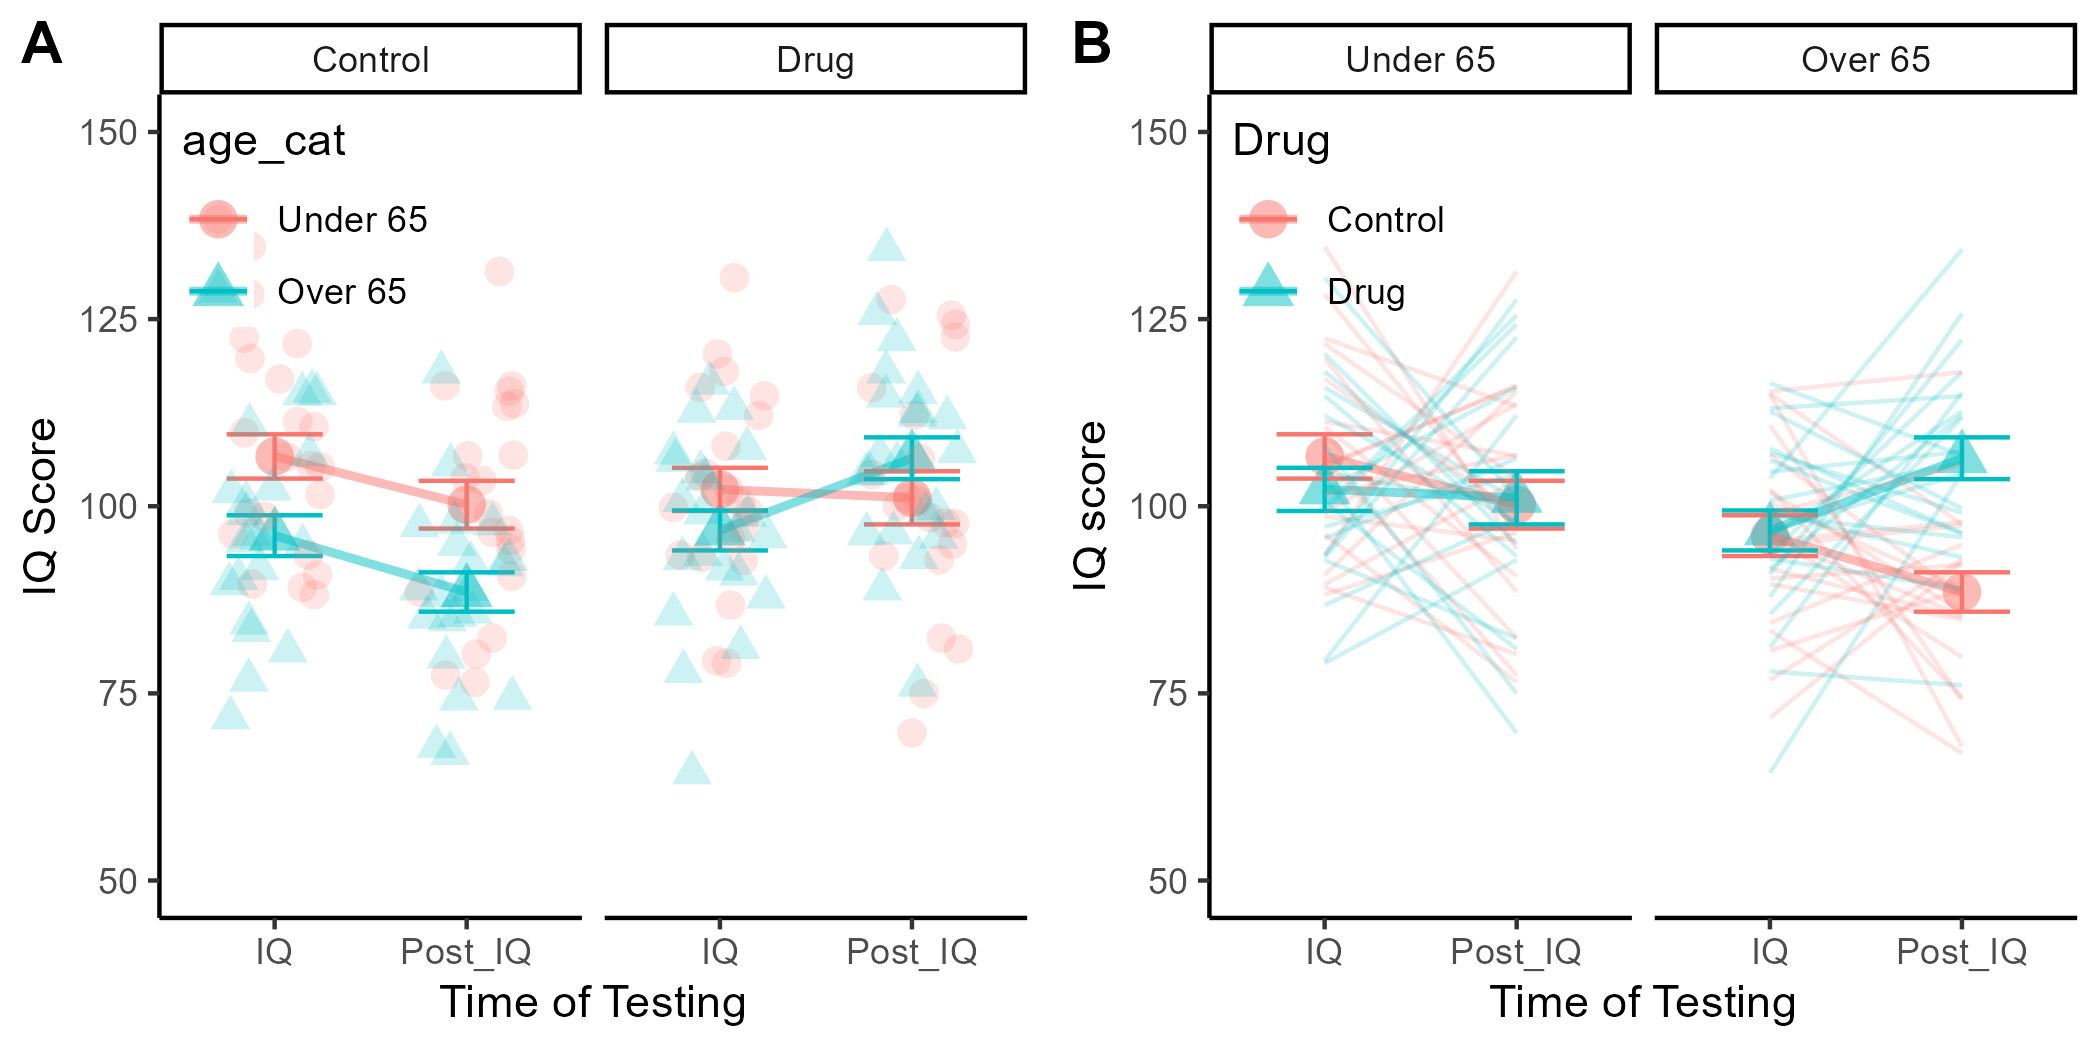
\includegraphics[width=29.17in]{graph_1}

\begin{Shaded}
\begin{Highlighting}[]
\CommentTok{\# Run a 3{-}way ANOVA to analyze your variables: }
\NormalTok{a }\OtherTok{\textless{}{-}} \FunctionTok{anova\_test}\NormalTok{(}\AttributeTok{data =}\NormalTok{ long\_data, }\AttributeTok{dv =}\NormalTok{ value, }\AttributeTok{within =}\NormalTok{ variable, }\AttributeTok{wid =}\NormalTok{ ID, }\AttributeTok{between =} \FunctionTok{c}\NormalTok{(age\_cat,Drug))}
\FunctionTok{get\_anova\_table}\NormalTok{(a)}
\end{Highlighting}
\end{Shaded}

\begin{verbatim}
## ANOVA Table (type III tests)
## 
##                  Effect DFn DFd     F     p p<.05   ges
## 1               age_cat   1  81 7.917 0.006     * 0.043
## 2                  Drug   1  81 3.576 0.062       0.020
## 3              variable   1  81 0.401 0.528       0.003
## 4          age_cat:Drug   1  81 7.639 0.007     * 0.042
## 5      age_cat:variable   1  81 1.263 0.264       0.008
## 6         Drug:variable   1  81 6.808 0.011     * 0.043
## 7 age_cat:Drug:variable   1  81 1.892 0.173       0.012
\end{verbatim}

\begin{itemize}
\tightlist
\item
  There is a significant main effect of age (F (1,81) = 7.92, p = 0.006).
\item
  There is a significant interaction between age and drug treatment (F(1,81) = 7.64, p = 0.007).
\item
  There is a significant interaction between drug treatment and time of testing (F(1,81) = 6.81, p = 0.01).
\end{itemize}

\subsection*{Follow up pair-wise comparisons}\label{follow-up-pair-wise-comparisons}
\addcontentsline{toc}{subsection}{Follow up pair-wise comparisons}

\begin{Shaded}
\begin{Highlighting}[]
\DocumentationTok{\#\# Always two ways to follow up: \#1:}
\NormalTok{long\_data }\SpecialCharTok{\%\textgreater{}\%}
  \FunctionTok{group\_by}\NormalTok{(age\_cat) }\SpecialCharTok{\%\textgreater{}\%}
  \FunctionTok{pairwise\_t\_test}\NormalTok{(value}\SpecialCharTok{\textasciitilde{}}\NormalTok{Drug)}
\end{Highlighting}
\end{Shaded}

\begin{verbatim}
## # A tibble: 2 x 10
##   age_cat  .y.   group1 group2    n1    n2       p p.signif   p.adj p.adj.signif
## * <fct>    <chr> <chr>  <chr>  <int> <int>   <dbl> <chr>      <dbl> <chr>       
## 1 Under 65 value Contr~ Drug      42    42 0.583   ns       0.583   ns          
## 2 Over 65  value Contr~ Drug      42    44 0.00155 **       0.00155 **
\end{verbatim}

\begin{itemize}
\tightlist
\item
  There was no effect of the drug on IQ scores for people that were under 65 (p = 0.58).
\item
  There was a significant effect of the drug treatment on IQ scores for people that were over 65 (p = 0.0016).
\end{itemize}

\begin{Shaded}
\begin{Highlighting}[]
\DocumentationTok{\#\# Number 2: }
\NormalTok{long\_data }\SpecialCharTok{\%\textgreater{}\%}
  \FunctionTok{group\_by}\NormalTok{(variable) }\SpecialCharTok{\%\textgreater{}\%}
  \FunctionTok{pairwise\_t\_test}\NormalTok{(value}\SpecialCharTok{\textasciitilde{}}\NormalTok{Drug)}
\end{Highlighting}
\end{Shaded}

\begin{verbatim}
## # A tibble: 2 x 10
##   variable .y.   group1 group2    n1    n2       p p.signif   p.adj p.adj.signif
## * <fct>    <chr> <chr>  <chr>  <int> <int>   <dbl> <chr>      <dbl> <chr>       
## 1 IQ       value Contr~ Drug      42    43 0.514   ns       0.514   ns          
## 2 Post_IQ  value Contr~ Drug      42    43 0.00383 **       0.00383 **
\end{verbatim}

\begin{itemize}
\tightlist
\item
  There was no difference in IQ scores between the experimental groups before treatment (i.e., at the first IQ measurement p = 0.51)
\item
  At the second IQ test, participants in the ``Drug'' group had higher IQ scores than participants in the control group p = 0.0039.
\end{itemize}

\subsection*{Linear Regression}\label{linear-regression}
\addcontentsline{toc}{subsection}{Linear Regression}

Compute, interpret, and graph the results of a multiple regression where the continuous covariate is entered as the predictor with the independent variable entered as the moderator. Interpret the linear relationships between the continuous covariate and the dependent variable at each level of your experimental treatment condition.

So far, we've worked with categorized versions of the covariate. But this was based on a construct that exists on a continuous scale in the real world (e.g., age, in my case). Now, run a linear regression of model the continuous relationship at the different levels of your independent variable.

\begin{Shaded}
\begin{Highlighting}[]
\CommentTok{\# Plot correlations between the continuous covariate and the DV for the two levels of your IV}
\NormalTok{A }\OtherTok{\textless{}{-}}\NormalTok{ final\_data }\SpecialCharTok{\%\textgreater{}\%}
  \FunctionTok{group\_by}\NormalTok{(Drug) }\SpecialCharTok{\%\textgreater{}\%}
  \FunctionTok{ggplot}\NormalTok{(}\FunctionTok{aes}\NormalTok{(}\AttributeTok{x=}\NormalTok{Age,}\AttributeTok{y=}\NormalTok{Post\_IQ)) }\SpecialCharTok{+}
  \FunctionTok{geom\_point}\NormalTok{(}\AttributeTok{size=}\DecValTok{4}\NormalTok{,}\AttributeTok{alpha=}\FloatTok{0.4}\NormalTok{)}\SpecialCharTok{+}
  \FunctionTok{geom\_smooth}\NormalTok{(}\AttributeTok{method=}\StringTok{"lm"}\NormalTok{)}\SpecialCharTok{+}
  \FunctionTok{facet\_wrap}\NormalTok{(}\SpecialCharTok{\textasciitilde{}}\NormalTok{Drug)}\SpecialCharTok{+}
  \FunctionTok{theme\_classic}\NormalTok{()}

\FunctionTok{ggsave}\NormalTok{(}\StringTok{"graph\_2.png"}\NormalTok{,A,}\AttributeTok{height=}\FloatTok{3.5}\NormalTok{,}\AttributeTok{width=}\DecValTok{6}\NormalTok{,}\AttributeTok{dpi=}\DecValTok{300}\NormalTok{)}
\NormalTok{knitr}\SpecialCharTok{::}\FunctionTok{include\_graphics}\NormalTok{(}\StringTok{"graph\_2.png"}\NormalTok{)}
\end{Highlighting}
\end{Shaded}

\begin{figure}
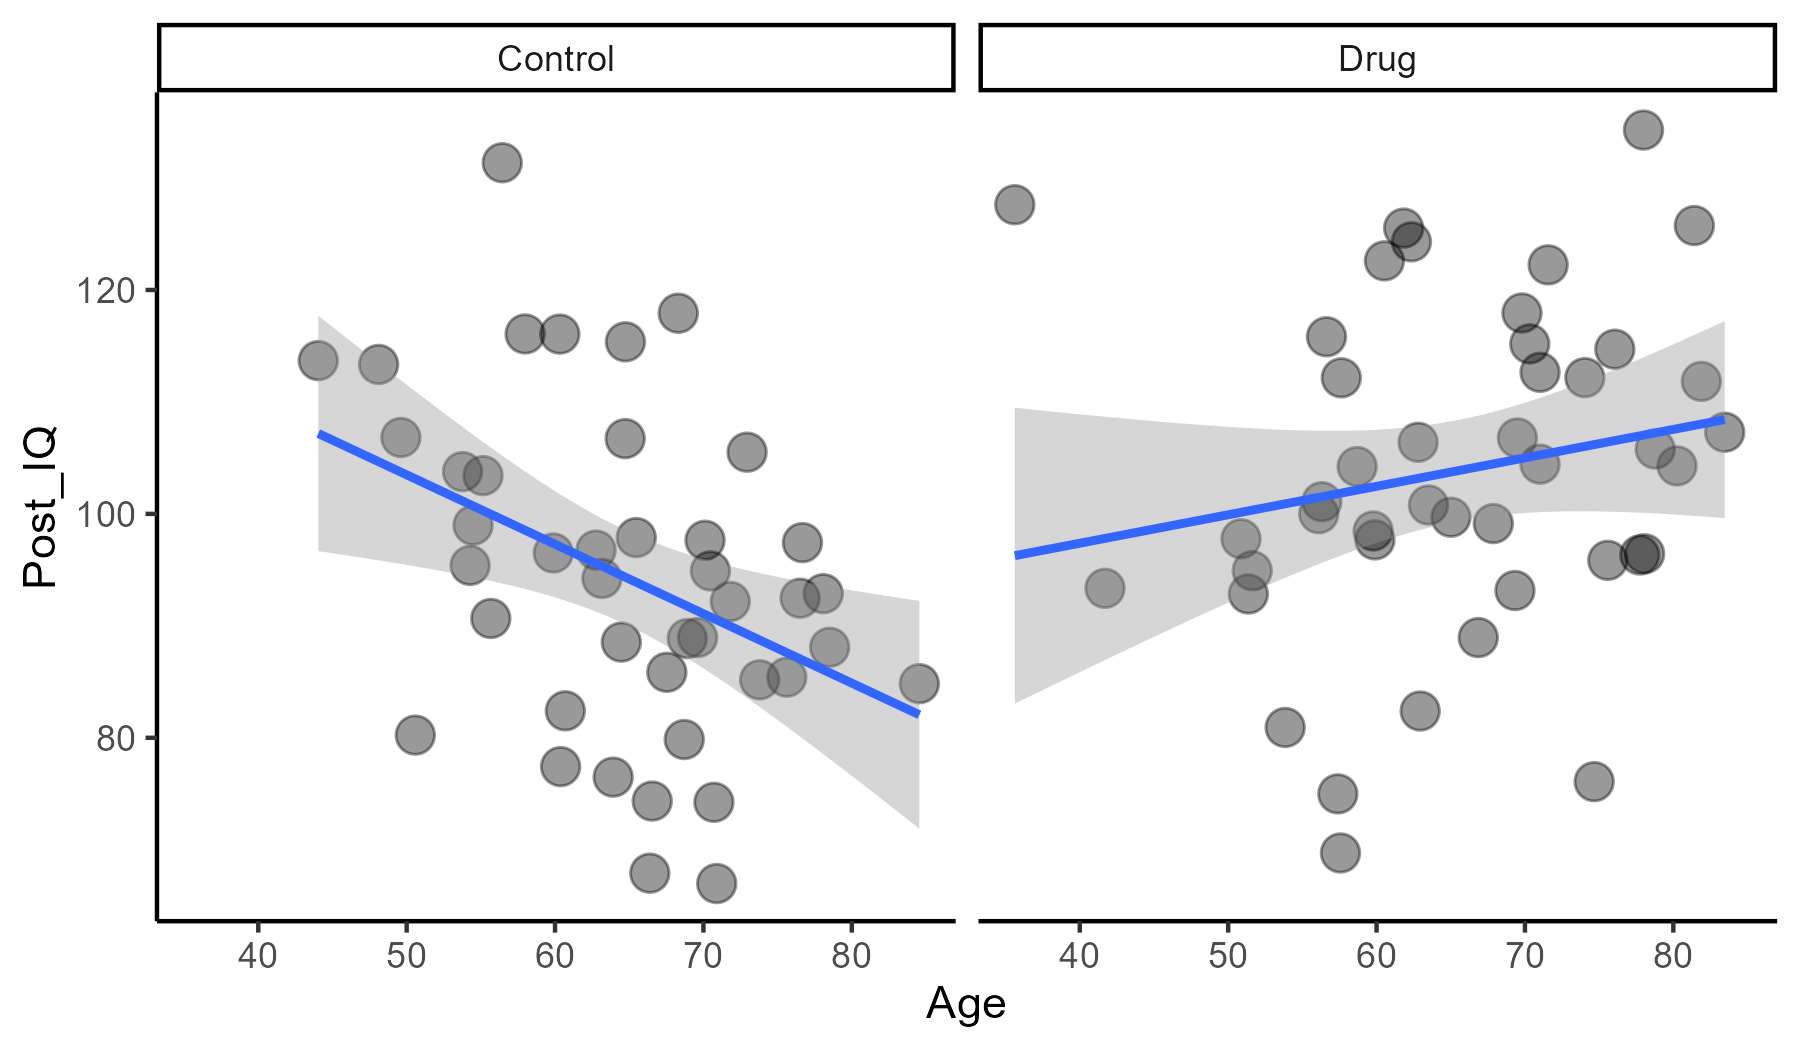
\includegraphics[width=25in]{graph_2} \caption{Side-by-side comparisons of continuous relationships at each level of the moderator.}\label{fig:unnamed-chunk-33}
\end{figure}

\begin{Shaded}
\begin{Highlighting}[]
\CommentTok{\# Be creative and choose a visual depiction that works for you! }
\NormalTok{B }\OtherTok{\textless{}{-}}\NormalTok{ final\_data }\SpecialCharTok{\%\textgreater{}\%}
  \FunctionTok{group\_by}\NormalTok{(Drug) }\SpecialCharTok{\%\textgreater{}\%}
  \FunctionTok{ggplot}\NormalTok{(}\FunctionTok{aes}\NormalTok{(}\AttributeTok{x=}\NormalTok{Age,}\AttributeTok{y=}\NormalTok{Post\_IQ,}\AttributeTok{colour=}\NormalTok{Drug,}\AttributeTok{fill=}\NormalTok{Drug,}\AttributeTok{shape=}\NormalTok{Drug))}\SpecialCharTok{+}
  \FunctionTok{geom\_point}\NormalTok{(}\AttributeTok{size=}\DecValTok{4}\NormalTok{,}\AttributeTok{alpha=}\FloatTok{0.4}\NormalTok{)}\SpecialCharTok{+}
  \FunctionTok{geom\_smooth}\NormalTok{(}\AttributeTok{method=}\StringTok{"lm"}\NormalTok{,}\AttributeTok{alpha=}\FloatTok{0.2}\NormalTok{)}\SpecialCharTok{+}
  \FunctionTok{theme\_classic}\NormalTok{()}\SpecialCharTok{+}
  \FunctionTok{theme}\NormalTok{(}\AttributeTok{legend.position =} \FunctionTok{c}\NormalTok{(}\DecValTok{0}\NormalTok{,}\DecValTok{1}\NormalTok{),}\AttributeTok{legend.justification =} \FunctionTok{c}\NormalTok{(}\DecValTok{0}\NormalTok{,}\DecValTok{1}\NormalTok{))}

\FunctionTok{ggsave}\NormalTok{(}\StringTok{"graph\_3.png"}\NormalTok{,B,}\AttributeTok{height=}\DecValTok{4}\NormalTok{,}\AttributeTok{width=}\DecValTok{4}\NormalTok{,}\AttributeTok{dpi=}\DecValTok{300}\NormalTok{)}
\NormalTok{knitr}\SpecialCharTok{::}\FunctionTok{include\_graphics}\NormalTok{(}\StringTok{"graph\_3.png"}\NormalTok{)}
\end{Highlighting}
\end{Shaded}

\begin{figure}
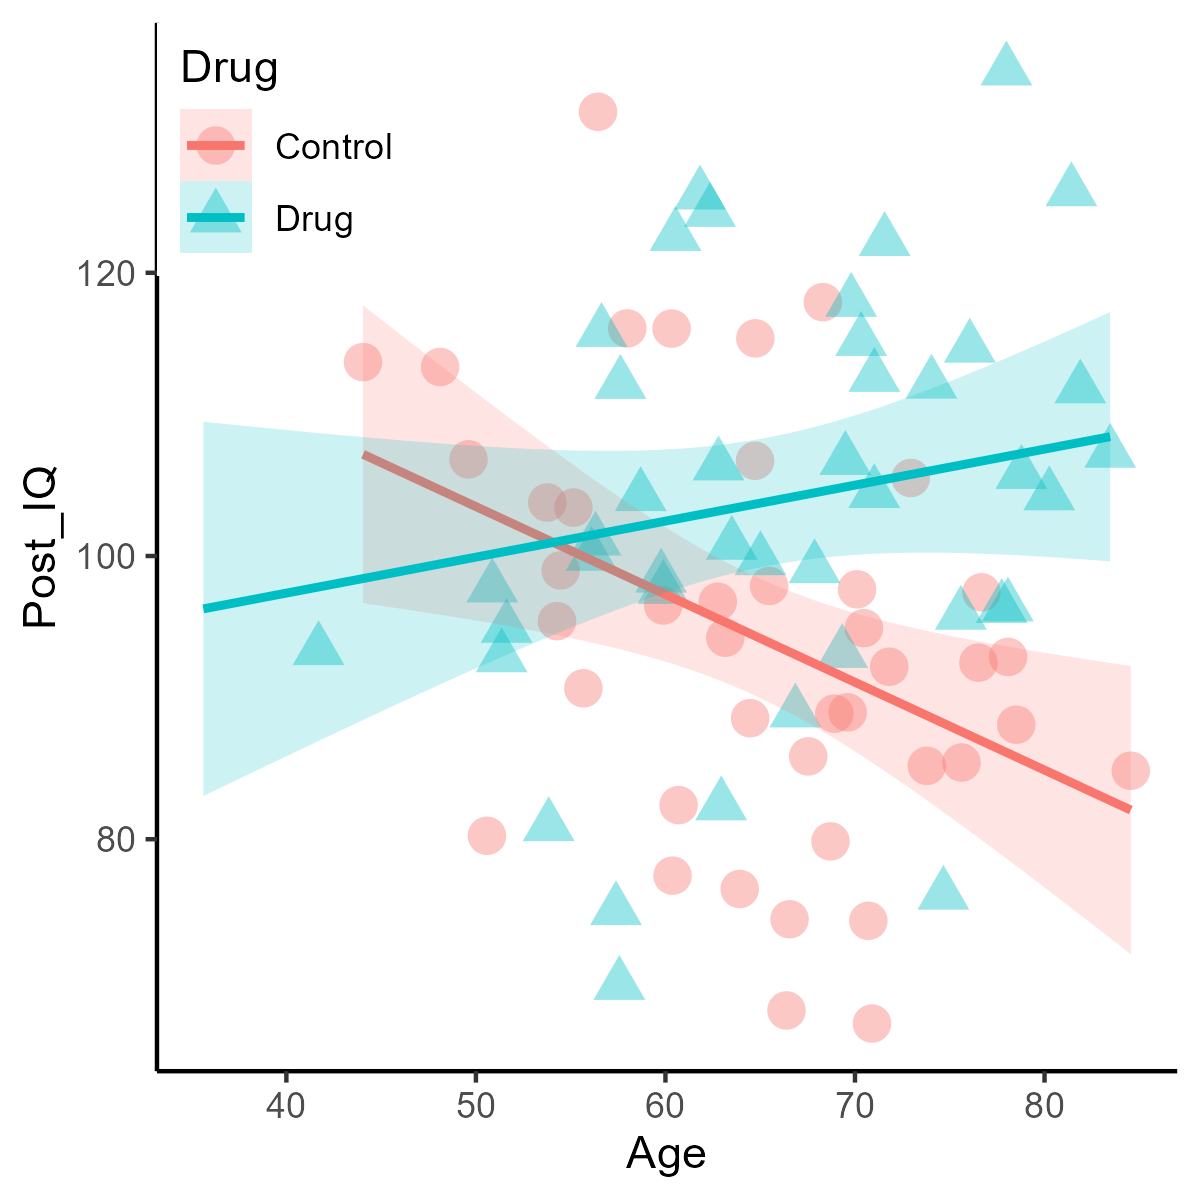
\includegraphics[width=16.67in]{graph_3} \caption{Overlapping lines show the different linear relationships for the two levels of the moderator variable.}\label{fig:unnamed-chunk-34}
\end{figure}

\begin{Shaded}
\begin{Highlighting}[]
\CommentTok{\# Run a linear regression to measure whether the continuous relationship between the covariate and the DV differs at the two levels of your independent variable during the "post{-}test" measurement. }
\NormalTok{baseline\_model }\OtherTok{\textless{}{-}} \FunctionTok{lm}\NormalTok{(}\AttributeTok{data =}\NormalTok{ final\_data, IQ }\SpecialCharTok{\textasciitilde{}}\NormalTok{ Age)}
\FunctionTok{summary}\NormalTok{(baseline\_model)}
\end{Highlighting}
\end{Shaded}

\begin{verbatim}
## 
## Call:
## lm(formula = IQ ~ Age, data = final_data)
## 
## Residuals:
##     Min      1Q  Median      3Q     Max 
## -33.851  -7.613  -0.847  10.302  33.607 
## 
## Coefficients:
##             Estimate Std. Error t value            Pr(>|t|)    
## (Intercept) 123.8054     9.2884   13.33 <0.0000000000000002 ***
## Age          -0.3600     0.1412   -2.55              0.0126 *  
## ---
## Signif. codes:  0 '***' 0.001 '**' 0.01 '*' 0.05 '.' 0.1 ' ' 1
## 
## Residual standard error: 13.01 on 83 degrees of freedom
## Multiple R-squared:  0.07267,    Adjusted R-squared:  0.0615 
## F-statistic: 6.504 on 1 and 83 DF,  p-value: 0.0126
\end{verbatim}

\begin{itemize}
\tightlist
\item
  At the baseline IQ test, the model predicts that a 1-year increase in age is associated with a 0.32-point decrease in IQ score.
\end{itemize}

\begin{Shaded}
\begin{Highlighting}[]
\CommentTok{\# Run a linear regression to measure whether the continuous relationship between the covariate and the DV differs at the two levels of your independent variable during the "post{-}test" measurement. }
\NormalTok{a }\OtherTok{\textless{}{-}} \FunctionTok{lm}\NormalTok{(}\AttributeTok{data =}\NormalTok{ final\_data, Post\_IQ }\SpecialCharTok{\textasciitilde{}}\NormalTok{ Age }\SpecialCharTok{*}\NormalTok{ Drug)}
\FunctionTok{summary}\NormalTok{(a)}
\end{Highlighting}
\end{Shaded}

\begin{verbatim}
## 
## Call:
## lm(formula = Post_IQ ~ Age * Drug, data = final_data)
## 
## Residuals:
##     Min      1Q  Median      3Q     Max 
## -32.131  -6.764  -0.849   7.384  31.873 
## 
## Coefficients:
##              Estimate Std. Error t value          Pr(>|t|)    
## (Intercept)  134.4990    15.7772   8.525 0.000000000000691 ***
## Age           -0.6202     0.2415  -2.568           0.01207 *  
## DrugDrug     -47.2863    20.5379  -2.302           0.02388 *  
## Age:DrugDrug   0.8744     0.3126   2.797           0.00643 ** 
## ---
## Signif. codes:  0 '***' 0.001 '**' 0.01 '*' 0.05 '.' 0.1 ' ' 1
## 
## Residual standard error: 14.13 on 81 degrees of freedom
## Multiple R-squared:  0.1798, Adjusted R-squared:  0.1494 
## F-statistic: 5.917 on 3 and 81 DF,  p-value: 0.001057
\end{verbatim}

\begin{itemize}
\tightlist
\item
  The model accounts for \textasciitilde18\% of the variability in IQ scores (F(3,81) = 5.92, p = 0.001).
\item
  The predicted IQ score for an individual that is 0 years old and did not receive the drug treatment is 134.499
\item
  A 1-year increase in age is associated with a 0.62-point decrease in IQ score among participants in the control group (t = 2.57, p = 0.012)
\item
  The relationship between age and IQ score was different at the two levels of drug treatment (t = 2.80, p = 0.006).
\end{itemize}

\begin{Shaded}
\begin{Highlighting}[]
\CommentTok{\# Check out the nature of the linear relationship between the continuous covariate and the DV at each level of your IV:}
\DocumentationTok{\#\# Control group first:}
\NormalTok{control\_only }\OtherTok{\textless{}{-}}\NormalTok{ final\_data[final\_data}\SpecialCharTok{$}\NormalTok{Drug }\SpecialCharTok{==} \StringTok{"Control"}\NormalTok{, ]}
\NormalTok{c }\OtherTok{\textless{}{-}} \FunctionTok{lm}\NormalTok{(}\AttributeTok{data =}\NormalTok{ control\_only, Post\_IQ }\SpecialCharTok{\textasciitilde{}}\NormalTok{ Age)}
\FunctionTok{summary}\NormalTok{(c)}
\end{Highlighting}
\end{Shaded}

\begin{verbatim}
## 
## Call:
## lm(formula = Post_IQ ~ Age, data = control_only)
## 
## Residuals:
##     Min      1Q  Median      3Q     Max 
## -25.418  -6.565   1.707   6.598  31.873 
## 
## Coefficients:
##             Estimate Std. Error t value        Pr(>|t|)    
## (Intercept) 134.4990    15.0797   8.919 0.0000000000469 ***
## Age          -0.6202     0.2308  -2.687          0.0105 *  
## ---
## Signif. codes:  0 '***' 0.001 '**' 0.01 '*' 0.05 '.' 0.1 ' ' 1
## 
## Residual standard error: 13.5 on 40 degrees of freedom
## Multiple R-squared:  0.1529, Adjusted R-squared:  0.1317 
## F-statistic: 7.218 on 1 and 40 DF,  p-value: 0.01046
\end{verbatim}

\begin{itemize}
\tightlist
\item
  Variability in age accounts for a statistically significant 15\% of the variability in IQ scores (R\^{}2 = 0.153, p = 0.01).
\item
  Same result as in the multiple regression model above :)
\item
  Information about the relationship between X \& Y in the ``reference'' group.
\end{itemize}

\begin{Shaded}
\begin{Highlighting}[]
\DocumentationTok{\#\# Then the drug group: }
\NormalTok{Drug\_only }\OtherTok{\textless{}{-}}\NormalTok{ final\_data[final\_data}\SpecialCharTok{$}\NormalTok{Drug }\SpecialCharTok{==} \StringTok{"Drug"}\NormalTok{, ]}
\NormalTok{d }\OtherTok{\textless{}{-}} \FunctionTok{lm}\NormalTok{(}\AttributeTok{data =}\NormalTok{ Drug\_only, Post\_IQ }\SpecialCharTok{\textasciitilde{}}\NormalTok{ Age)}
\FunctionTok{summary}\NormalTok{(d)}
\end{Highlighting}
\end{Shaded}

\begin{verbatim}
## 
## Call:
## lm(formula = Post_IQ ~ Age, data = Drug_only)
## 
## Residuals:
##     Min      1Q  Median      3Q     Max 
## -32.131  -6.412  -1.443   9.133  31.348 
## 
## Coefficients:
##             Estimate Std. Error t value    Pr(>|t|)    
## (Intercept)  87.2127    13.6920    6.37 0.000000129 ***
## Age           0.2542     0.2066    1.23       0.226    
## ---
## Signif. codes:  0 '***' 0.001 '**' 0.01 '*' 0.05 '.' 0.1 ' ' 1
## 
## Residual standard error: 14.71 on 41 degrees of freedom
## Multiple R-squared:  0.0356, Adjusted R-squared:  0.01207 
## F-statistic: 1.513 on 1 and 41 DF,  p-value: 0.2256
\end{verbatim}

\begin{itemize}
\tightlist
\item
  Variability in age only accounts for 3\% of variability in IQ scores, which is not statistically significant (p = 0.226).
\item
  Among drug-treated participants, age is no longer a significant predictor of IQ (p = 0.226).
\item
  Moreover, the (non-statistically-significant) estimate is positive for the drug group (b = 0.25).
\end{itemize}

\section*{Discussion}\label{discussion}
\addcontentsline{toc}{section}{Discussion}

Unpack / explain the results from your current simulated experiment in the context of the literature that you cited in your introduction. What would these findings indicate? Why would they be important? In what ways would this finding be meaningful? What would these results indicate about the constructs that you are aiming to capture?

Please also explain what grouping the covariate into categories (and running factorial ANOVA) versus using linear regression on the continuous covariate add to your understanding of the measured variables.

The discussion should be between 1000 - 2000 words. Focus on \textbf{\emph{quality}} rather than quantity. Subheadings are often useful in the discussion section. Use subheadings in such a way that they enhance your narrative. Make sure that you are \textbf{\emph{discussing}} the findings (i.e., don't just re-state the results).

Here, you should also reflect on the strengths and weaknesses of your current approach. Connect your theoretical study to real-world scenarios. Should this research be carried out in real life? Why or why not? Are there other, more logical or feasible versions of this experiment that should or could be conducted? Any thoughts about experimental design for future researchers?

\subsection*{Conclusions}\label{conclusions}
\addcontentsline{toc}{subsection}{Conclusions}

\begin{itemize}
\tightlist
\item
  Drug treatment does not improve IQ on its own, but it seems to reverse age-related cognitive declines on the IQ test.
\end{itemize}

\section*{References}\label{references}
\addcontentsline{toc}{section}{References}

List your references in alphabetical order, using internal APA format (no hanging indents).

\chapter*{TA Responsibilities}\label{ta-responsibilities}
\addcontentsline{toc}{chapter}{TA Responsibilities}

\section*{Overview}\label{overview-2}
\addcontentsline{toc}{section}{Overview}

\begin{itemize}
\tightlist
\item
  Anticipated enrollment = 38 students
\end{itemize}

The assignments build across the term, so it makes the most sense for \textbf{each TA to be assigned \textasciitilde13 students} to assess throughout the term.

\begin{itemize}
\tightlist
\item
  We will split the two term tests such that each of you grades 1-2 questions across all of the tests.
\end{itemize}

\section*{Course Deliverables}\label{course-deliverables}
\addcontentsline{toc}{section}{Course Deliverables}

\subsection*{1. 5x 3\% ``Practical'' assignments}\label{x-3-practical-assignments}
\addcontentsline{toc}{subsection}{1. 5x 3\% ``Practical'' assignments}

\begin{itemize}
\tightlist
\item
  Each TA marks bi-weekly submissions for \textasciitilde13 students.
\item
  Practicals are intended to be ``bite-sized'' pieces of their final paper project.
\item
  Each submission will be graded out of 15 marks.
\item
  A rubric will be provided on Quercus to evaluate the practical submissions.
\end{itemize}

\subsection*{2. 2x 25\% Tests}\label{x-25-tests}
\addcontentsline{toc}{subsection}{2. 2x 25\% Tests}

\begin{itemize}
\tightlist
\item
  Completed on Quercus
\item
  MC will be auto-graded
\item
  Answer keys for SA questions will be provided the day of the test.
\end{itemize}

\subsection*{3. 5\% Poster Presentation}\label{poster-presentation}
\addcontentsline{toc}{subsection}{3. 5\% Poster Presentation}

\begin{itemize}
\tightlist
\item
  The purpose of this assignment is to encourage students to complete and understand their analysis for the final project well ahead of the deadline to submit the written report.
\item
  Students will upload a 5-minute video explaining their project and results.
\item
  Mostly graded for completion, but also offers an opportunity to provide feedback about the interpretations.
\end{itemize}

\subsection*{3. 20\% Paper}\label{paper}
\addcontentsline{toc}{subsection}{3. 20\% Paper}

\begin{itemize}
\tightlist
\item
  ``Capstone'' project for this course (12-14 pages all-in)
\item
  You will evaluate the same \textasciitilde13 students as you have graded all semester.
\item
  A detailed rubric will be provided on Quercus to evaluate the essays.
\end{itemize}

\subsection*{4. 10\% In-class participation}\label{in-class-participation}
\addcontentsline{toc}{subsection}{4. 10\% In-class participation}

\begin{itemize}
\tightlist
\item
  No contribution from TAs - Jennet will manage.
\end{itemize}

\subsection*{TA Student contact}\label{ta-student-contact}
\addcontentsline{toc}{subsection}{TA Student contact}

\begin{itemize}
\item
  10 weekly office hours - \textbf{Please send Jennet your personal zoom links}
\item
  Remaining hours allocated to student contact in the DDAH form can be used to field emails.
\item
  In any situation where students are hostile or you don't know how to respond to them, feel free to forward their correspondences along to me to deal with. \emph{You can count on me to back up your calls!}
\end{itemize}

\section*{Course Responsibilities}\label{course-responsibilities}
\addcontentsline{toc}{section}{Course Responsibilities}

All of your TA responsibilities can be completed virtually. Psy309 will involve two in-class tests that will be completed on Quercus.

\begin{tabular}{l|l|l|l}
\hline
Assignment & Due\_Date & Format & Size\\
\hline
Practical 1 & 2024-09-13 & Online & Small\\
\hline
Practical 2 & 2024-09-27 & Online & Small\\
\hline
Test \#1 & 2024-10-04 & Online & Med\\
\hline
Practical 3 & 2024-10-11 & Online & Small\\
\hline
Practical 4 & 2024-10-25 & Online & Small\\
\hline
Practical 5 & 2024-11-08 & Online & Small\\
\hline
Poster & 2024-11-15 & Online & Small\\
\hline
Test \#2 & 2024-11-22 & Online & Med\\
\hline
Paper & 2024-12-03 & Online & Largest\\
\hline
\end{tabular}

\emph{Note} That there will be late / deferred submissions for all of the assignments.

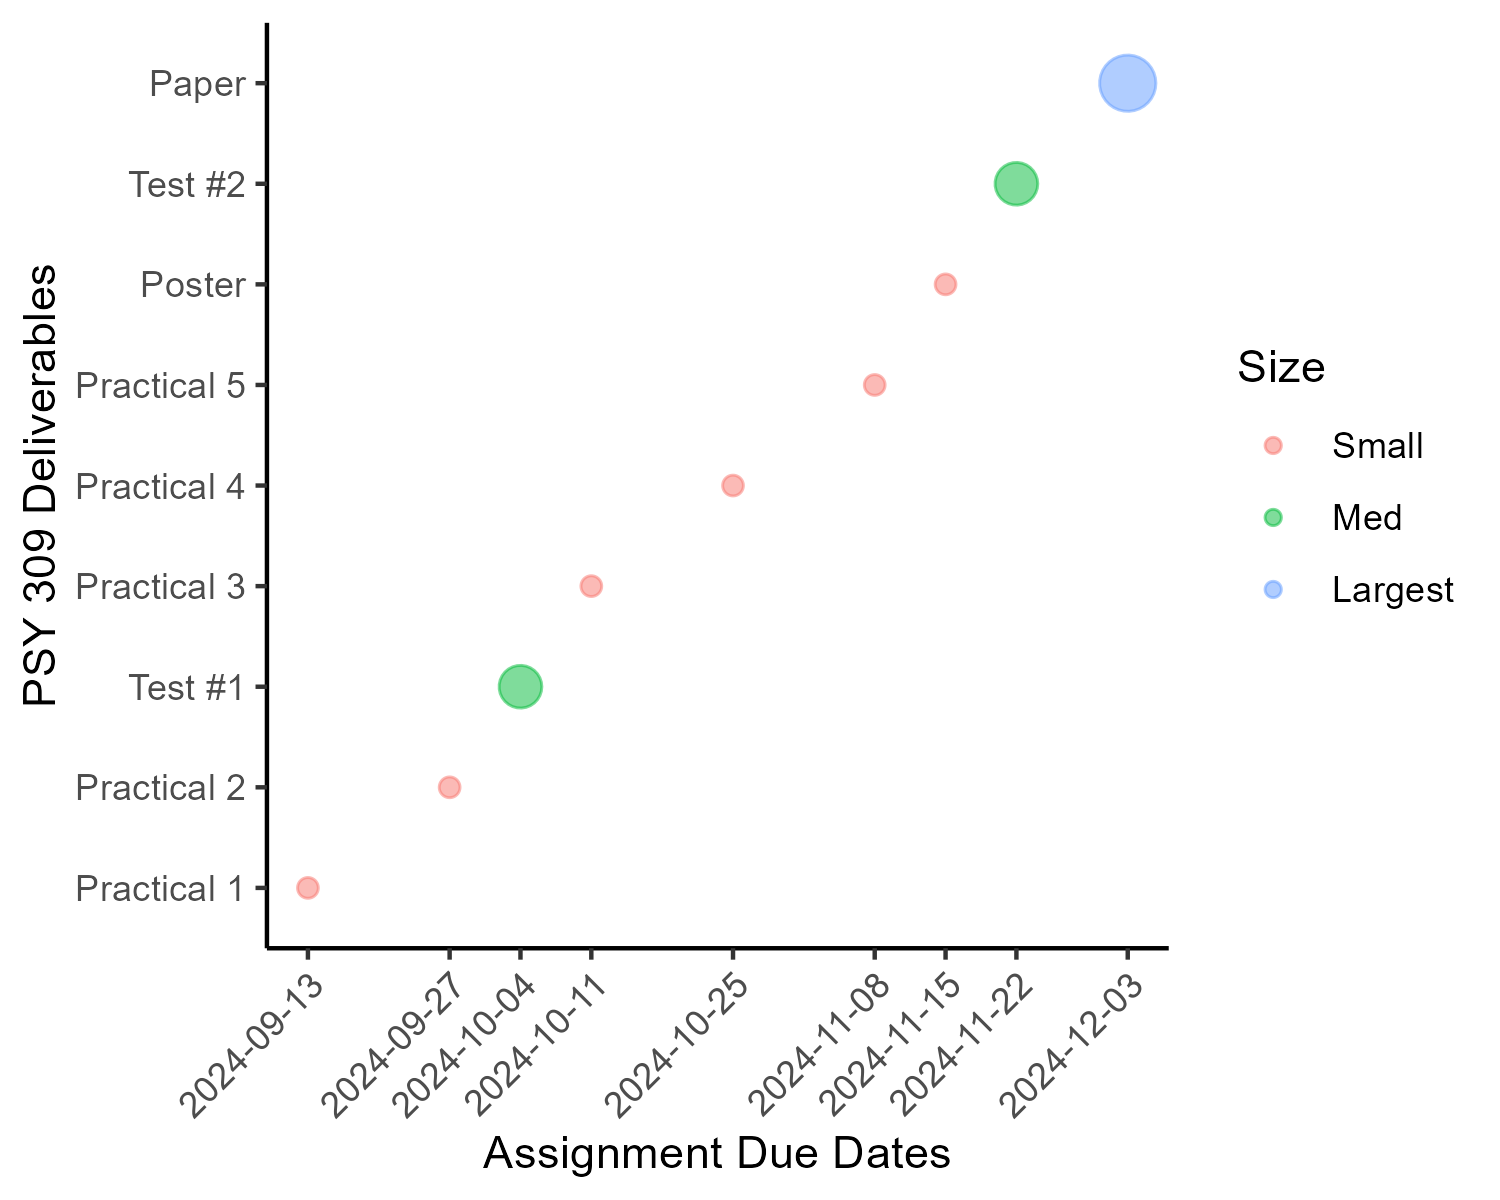
\includegraphics[width=20.83in]{Psy309_deliverables}

\subsection*{Reminders}\label{reminders}
\addcontentsline{toc}{subsection}{Reminders}

\begin{itemize}
\tightlist
\item
  Practical assignments are due Fridays at 11:59pm.
\end{itemize}

I will email you a reminder that submissions are available the day after the due date.

\end{document}
